
%\documentclass[11pt]{beamer}
\documentclass[12pt,xcolor=pdflatex,dvipsnames,table]{beamer}
\usepackage[utf8]{inputenc}
\usepackage[czech]{babel}
\usepackage{amsthm}
\usepackage{amssymb}
\usepackage{amsmath}
\usepackage{array}
\usepackage{stmaryrd}
\usepackage{graphicx}
\usepackage{tabularx}
\usepackage{listings}
\usepackage{fancyvrb}
\usepackage{minted}



\theoremstyle{definition}
\newtheorem{indefinition}{Definition}

\theoremstyle{example}
\newtheorem{inexample}{Example}

\theoremstyle{denotation}
\newtheorem{indenotation}{Denotation}

\theoremstyle{theorem}
\newtheorem{intheorem}{Theorem}

%\title{Strukturni rozpoznávání, extrakce a analýza příznaků z textur}
\title{Pokročilá práce se shadery, Bindless Textury, DSA, Teselace, Compute Shader}
\institute[VUT FIT]{Ústav počítačové grafiky a multimédií\\Fakulta informačních technologií\\Vysoké učení technické Brno}
\author[Tomáš Milet]{Tomáš Milet}
\date{\today}

\mode<presentation>
{
    \usetheme{FIT}
}

\begin{document}

\begin{frame}
\titlepage
\end{frame}

\begin{frame}

\frametitle{Buffery}
	\begin{itemize}
		\item Buffer je paměť na GPU
		\item Unikátní celočíselný identifikátor
		\item Může být připojen na různá místa VBO, EBO, ...
		\item Několik způsobů zápisu a používání
		\item Zápis/čtení z CPU/GPU
	\end{itemize}
\end{frame}


\begin{frame}
\frametitle{Použití Buffer}
    \begin{enumerate}
        \item{Získání jména Bufferu.}
				\item{Vytvoření Bufferu}
				\item{Alokace místa pro Buffer}
				\item{Nahrání dat do Buffer}
				\item{Připojení Bufferu}
				\item{Uvolnění Buffer.}
    \end{enumerate}
\end{frame}


\begin{frame}[fragile]

\frametitle{Vytvoření/uvolnění identifikátorů}
	\begin{itemize}
		\item{Pomocí identifikátoru (jména) komunikujeme s buffery.}
		\item{
		Vytvoření identifikátorů:\\
		{\scriptsize
		\mint[frame=lines]{c++}|void glGenBuffers(GLsizei n,GLuint * buffers);|
		}
		\begin{description}
			\item[n] Počet identifikátorů (jmen), které chceme vytvořit
			\item[buffers] Pole idenifikátorů
		\end{description}
		}

		\item{
		Uvolnění identifikátorů:\\
		{\scriptsize
		\mint[frame=lines]{c++}|void glDeleteBuffers(GLsizei n,GLuint * buffers);|
		}}

		\item{
		Funkce {\color{blue}glGenBuffers} má podobnou funkcionalitu jako funkce {\color{blue}glGenTextures}.
		}
	\end{itemize}
\end{frame}

\begin{frame}
\frametitle{Připojení Bufferu k targetu}
	\begin{itemize}

		\item{ Aktivování bufferu - touto funkcí určíme buffer, se kterým budeme pracovat dany target:\\
		{\scriptsize
		\mint[frame=lines]{c++}|void glBindBuffer(GLenum target,GLuint buffer);|
		}
		\begin{description}
			\item[target] Určuje typ bufferu a způsob jeho používání.
			\item[buffer] Identifikátor (jméno) bufferu.
		\end{description}
		}

	\end{itemize}
\end{frame}

\begin{frame}
\frametitle{Připojení Bufferu k targetu}
	\begin{figure}[h]
	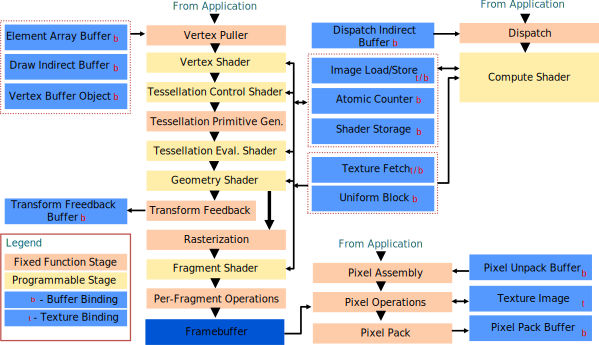
\includegraphics[width=11cm,keepaspectratio]{pics/opengl43.pdf}
	\end{figure}
\end{frame}


\begin{frame}
\frametitle{glBindBuffer() - hodnoty parametru target}
		\begin{description}
			\item[GL\_ARRAY\_BUFFER] Bufferu bude sloužit jako zdroj vrcholových dat
			\item[GL\_ELEMENT\_ARRAY\_BUFFER] Buffer bude sloužit jako indexy
			\item[GL\_ATOMIC\_COUNTER\_BUFFER] Buffer bude sloužit jako atomický čítač
			\item[GL\_DRAW\_INDIRECT\_BUFFER] Buffer bude sloužit pro indirect draw příkazy
			\item[...] ...
		\end{description}
\end{frame}

\begin{frame}[fragile]
\frametitle{Alokace Bufferu}
	\begin{itemize}

		\item{ Alokování bufferu - touto funkcí alokujeme buffer. Případně do něj můžeme nahrát data:\\
		{\scriptsize
		\begin{minted}[frame=lines]{c++}
		void glBufferData(GLenum target,GLsizeiptr size,
		                  const GLvoid*data,GLenum usage);
		\end{minted}
		}
		\begin{description}
			\item[target] Stejné jako u {\color{blue} glBindBuffer}.
			\item[size] Velikost bufferu v bajtech.
			\item[data] Ukazatel na data, která chceme nahrát.
			Při {\color{blue} NULL} se žádná data nekopírují.
			\item[usage] Způsob použití bufferu.
			Tímto parametrem sdělíme OpenGL, jakým způsobem budeme buffer používat.
			OpenGL zvolí nejvýhodnější alokaci bufferu z pohledu výkonnosti.
		\end{description}
		}

	\end{itemize}
\end{frame}

\begin{frame}
\frametitle{glBufferData() - hodnoty parametru usage}
	\begin{itemize}
		\item{Hodnoty GL\_X\_Y, kde X a Y je:}
		{\scriptsize
		\begin{tabular}{|l|l|}
		\hline
		X & popis \\ \hline
		STREAM & Data budou nahrána 1x a použita párkrát \\ \hline
		STATIC & Data budou nahrána 1x a použita mnohokrát \\ \hline
		DYNAMIC & Nahrání i používání dat bude časté \\ \hline
		\end{tabular}
		\begin{tabular}{|l|l|}
		\hline
		Y & popis \\ \hline
		DRAW & Data budou nahrána aplikací, vykreslení pomocí OpenGL \\ \hline
		READ & Data budou nahrána z OpenGL, aplikace čte data z VBO \\ \hline
		COPY & Data budou nahrána z OpenGL, vykreslení pomocí OpenGL \\ \hline
		\end{tabular}
		}
		\item{Hodnota parametru usage nijak neomezuje použití VBO.}
	\end{itemize}
\end{frame}

\begin{frame}[fragile]
\frametitle{Nahrání dat do Buffer}
	\begin{itemize}

		\item{ Funkcí pro alokaci dat můžeme také nahrát data.
		{\scriptsize
		\begin{minted}[frame=lines]{c++}
		void glBufferData(GLenum target,GLsizeiptr size,
		                  const GLvoid*data,GLenum usage);
		\end{minted}
		}}

		\item{ Nahrazení části bufferu novými daty.
		{\scriptsize
		\begin{minted}[frame=lines]{c++}
		void glBufferSubData(GLenum target,GLintptr offset,
		                     GLsizeiptr size,const GLvoid*data);
		\end{minted}
		}
		\begin{description}
		\item[target] Stejné jako u {\color{blue} glBindBuffer}.
		\item[offset] Offset v bajtech od začátku.
		\item[size] Velikost dat v bajtech
		\item[data] Ukazatel na data.
		\end{description}
		}
		{\scriptsize
		\begin{minted}[frame=lines]{c++}
		void glClearBufferData(GLenum target,GLenum internalformat,
		  GLenum format,GLenum type,const void * data);
		\end{minted}
		}
	\end{itemize}
\end{frame}

\begin{frame}[fragile]
\frametitle{Nahrání dat do Buffer}
	\begin{itemize}

		\item{ Touto funkcí můžeme 'vytáhnout' ukazatel na data v Bufferu.
		{\scriptsize
		\begin{minted}[frame=lines]{c++}
		void * glMapBuffer(GLenum target,GLenum access);
		\end{minted}
		}
		\begin{description}
		\item[target] Stejné jako u {\color{blue} glBindBuffer}.
		\item[access] Specifikuje přístup. Hodnoty GL\_READ\_ONLY, GL\_WRITE\_ONLY a GL\_READ\_WRITE.
		\end{description}
		}
		\item{ Po použití je potřeba uvolnit ukazatel.
		{\scriptsize
		\begin{minted}[frame=lines]{c++}
		GLboolean glUnmapBuffer(GLenum target);
		\end{minted}
		}}

	\end{itemize}
\end{frame}

\begin{frame}[fragile]
\frametitle{Příklad kódu}
	\begin{itemize}
		{\scriptsize
		\begin{minted}[frame=lines]{c++}
		float Data[]={0,0};//data, ktera budeme vkladat do bufferu
		GLuint VBO;//identifikator VBO
		glGenBuffers(1,&VBO);//vygenerujeme si identifikator
		glBindBuffer(GL_ARRAY_BUFFER,VBO);//aktivujeme si VBO
		//alokujeme buffer a nahrajeme do nej data
		glBufferData(GL_ARRAY_BUFFER,sizeof(Data),Data,GL_STATIC_DRAW);
		\end{minted}
		}
		Změna dat ve VBO.
		{\scriptsize
		\begin{minted}[frame=lines]{c++}
		float*ptr;//ukazatel na data
		ptr=(float*)glMapBuffer(GL_ARRAY_BUFFER,GL_READ_WRITE);//ziskame jej
		ptr[0]=0.5;//nastavime hodnotu prvniho prvku
		glUnmapBuffer(GL_ARRAY_BUFFER);//odmapujeme buffer
		\end{minted}
		}
		Nebo pomoci {\color{blue} glBufferSubData}.
		{\scriptsize
		\begin{minted}[frame=lines]{c++}
		glBufferSubData(GL_ARRAY_BUFFER,
		  sizeof(float),//nahrajeme nova s offsetem jeden float
		  sizeof(float),//nahrajeme jen jeden float
		  Data);//data
		\end{minted}
		}

	\end{itemize}
\end{frame}

\begin{frame}[fragile]
\frametitle{Vykreslení dat - získání identifikátoru atributu}
	\begin{itemize}
		\item{Vertex Shader:
		{\scriptsize
		\begin{minted}[frame=lines]{glsl}
		#version 330
		in vec2 inPos;//souradnice vertexu
		void main(){
		  gl_Position=vec4(inPos,0,1);
		}
		\end{minted}
		}}

		\item{Získání identifikátoru atributu z shaderu.
		{\scriptsize
		\begin{minted}[frame=lines]{c++}
		GLint inPosAttrib;//identifikator atributu
		inPosAttrib=glGetAttribLocation(
		  Shader,//shader program
		  "inPos");//nazev vstupni promenne v shaderu
		\end{minted}
		}}

	\end{itemize}
\end{frame}

\begin{frame}[fragile]
\frametitle{Vykreslení dat - navázání/aktivování atributu}
	\begin{itemize}
		\item{Před samotným vykreslením je potřeba navázat atributy na VBO.
		{\scriptsize
		\begin{minted}[frame=lines]{c++}
		void glVertexAttribPointer(GLuint index,GLint size,GLenum type,
		GLboolean normalized,GLsizei stride,const GLvoid * pointer);
		\end{minted}
		}
		\begin{description}
		\item[index] Identifikátor atributu získaný funkcí {\color{blue} glGetAttribLocation}
		\item[size] Počet komponent na atribut 1-4.
		\item[type] Datový typ GL\_FLOAT, GL\_INT, ...
		\item[normalized] normalizace GL\_FALSE, GL\_TRUE
		\item[stride] rozestup v bajtech
		\item[pointer] Offset v bajtech
		\end{description}
		}
		\item{Aktivování/deaktivování atributu
		{\scriptsize
		\begin{minted}[frame=lines]{c++}
		void glEnableVertexAttribArray(GLuint index);
		\end{minted}
		}
		{\scriptsize
		\begin{minted}[frame=lines]{c++}
		void glDisableVertexAttribArray(GLuint index);
		\end{minted}
		}}
	\end{itemize}
\end{frame}

\begin{frame}[fragile]
\frametitle{Navázání atributů k VBO Příklad (1)}
	\begin{itemize}
		\item{Předpokládejme, že budeme k jednomu vrcholu ukládat 4 atributy.
		Pozici (A), čas (B), barvu (C), texturovací koordináty (D).
		\begin{figure}[h]
		\includegraphics[width=10cm,keepaspectratio]{pics/stride.pdf}
		%\caption{Výpočet koeficinetu $a_2$}
		%\label{a2}
		\end{figure}
		}
	\end{itemize}
\end{frame}

\begin{frame}[fragile]
\frametitle{Navázání atributů k VBO Příklad (2)}
	\begin{itemize}
		\item{Shader program:
		{\scriptsize
		\begin{minted}[frame=lines]{glsl}
		#version 330
		in vec3 A;//souradnice vertexu
		in float B;//cas
		in vec3 C;//barva
		in vec2 D;//texturovaci koordinaty
		void main(){
			//...
		}
		\end{minted}
		}}

		\item{Aplikace:
		{\scriptsize
		\begin{minted}[frame=lines]{c++}
		GLint Aatt=glGetAttribLocation(Shader,"A");
		//...
		glEnableVertexAttribArray(Aattrib);
		//...
		glVertexAttribPointer(Aatt,3,GL_FLOAT,GL_FALSE,sizeof(float)*9,(GLvoid*)0);
		glVertexAttribPointer(Batt,1,GL_FLOAT,GL_FALSE,sizeof(float)*9,
		  (GLvoid*)(sizeof(float)*3));
		glVertexAttribPointer(Catt,3,GL_FLOAT,GL_FALSE,sizeof(float)*9,
		  (GLvoid*)(sizeof(float)*4));
		glVertexAttribPointer(Datt,2,GL_FLOAT,GL_FALSE,sizeof(float)*9,
		  (GLvoid*)(sizeof(float)*7));
		\end{minted}
		}}

	\end{itemize}
\end{frame}

\begin{frame}[fragile]
\frametitle{Vykreslení dat}
	\begin{itemize}
		\item{Data můžeme z VBO vykreslovat pomocí dvou způsobů - Přímo nebo indexovaně.}
		\item{Přímý způsob vykreslování:
		{\scriptsize
		\begin{minted}[frame=lines]{c++}
		void glDrawArrays(GLenum mode,GLint first,GLsizei count);
		\end{minted}
		}
		\begin{description}
		\item[mode] Typ primitiva: GL\_POINTS, GL\_LINE\_STRIP,GL\_LINE, ...
		\item[first] Počáteční index (první vrchol)
		\item[count] Počet indexů (počet vrcholů)
		\end{description}
		}
	\end{itemize}
\end{frame}

\begin{frame}[fragile]
\frametitle{Vykreslení dat}
	\begin{itemize}
		\item{Pro vykreslování s indexováním budeme potřebovat další buffer - Element buffer object (EBO). Buffer bude obsahovat indexy.
		{\scriptsize
		\begin{minted}[frame=lines]{c++}
		unsigned Data[]={0,1,1,3,0};//indexy
		GLuint EBO;//identifikator EBO
		glGenBuffers(1,&EBO);//vygenerujeme si identifikator
		glBindBuffer(GL_ELEMENT_ARRAY_BUFFER,EBO);//aktivujeme si EBO
		glBufferData(GL_ELEMENT_ARRAY_BUFFER,sizeof(Data),Data,GL_STATIC_DRAW);
		\end{minted}
		}}
		\item{Vykreslování s indexováním je vhodné například k ušetření místa - 
		několik polygonů sdílí stejný vrchol.
		}
		\item{ Kreslící funkce:
		{\scriptsize
		\begin{minted}[frame=lines]{c++}
		void glDrawElements(GLenum mode,GLsizei count,GLenum type,
		  const GLvoid * indices);
		\end{minted}
		}
		{\scriptsize
		\begin{minted}[frame=lines]{c++}
		void glDrawRangeElements(GLenum mode,GLuint start,GLuint end,
		  GLsizei count,GLenum type,const GLvoid * indices);
		\end{minted}
		}
		}
	\end{itemize}
\end{frame}

\begin{frame}[fragile]
\frametitle{glDrawElements()}
	\begin{itemize}
		{\scriptsize
		\begin{minted}[frame=lines]{c++}
		void glDrawElements(GLenum mode,GLsizei count,GLenum type,
		  const GLvoid * indices);
		\end{minted}
		}
		\begin{description}
		\item[mode] Typ vykreslovaného primitiva GL\_POINTS,GL\_LINES,...
		\item[count] Počet indexů (vrcholů), které chceme vykreslit.
		Pro jeden trojúhelník je toto číslo 3.
		\item[type] Typ indexu GL\_UNSIGNED\_BYTE, GL\_UNSIGNED\_SHORT, GL\_UNSIGNED\_INT.
		Čím menší typ zvolíme, tím bude kreslení rychlejší.
		\item[indices] Offset v bajtech - od kterého indexu se bude kreslit.
		\end{description}


	\end{itemize}
\end{frame}

\begin{frame}[fragile]
\frametitle{Kompletní příklad - shader}
		Vertex Shader:
		{\scriptsize
		\begin{minted}[frame=lines]{glsl}
		#version 330
		in vec2 vPos;//pozice
		in vec3 vCol;//barva vstup
		out vec3 fCol;//brava do fragment shaderu
		void main(){
		  gl_Position=vec4(vPos,0,1);
		  fCol=vCol;
		}
		\end{minted}
		}
		Fragment Shader:
		{\scriptsize
		\begin{minted}[frame=lines]{glsl}
		#version 330
		layout(location=0)out vec4 fragColor;//vystup
		in vec3 fCol;//barva
		void main(){
		  fragColor=vec4(fCol,1);
		}
		\end{minted}
		}
\end{frame}
%
\begin{frame}[fragile]
\frametitle{Kompletní příklad - aplikace}
		Aplikace - inicializace:
		{\scriptsize
		\begin{minted}[frame=lines]{c++}
		GLint vPos=glGetAttribLocation(Shader,"vPos");//ident. pozice
		GLint vCol=glGetAttribLocation(Shader,"vCol");//ident. barvy
		float Data[]={//pozice, barva
		   .0, .0,   1,0,1,
		  -.5, .5,   1,0,0,
		  -.5,-.5,   0,1,1,
		  -1,  .0,   1,0,0
		};
		glGenBuffers(1,&VBO);//jmeno pro VBO
		glBindBuffer(GL_ARRAY_BUFFER,VBO);//aktivujeme VBO
		glBufferData(GL_ARRAY_BUFFER,sizeof(Data),Data,GL_STATIC_DRAW);//data
		unsigned Index[]={0,1,2,2,1,3};//indexy
		glGenBuffers(1,&EBO);//jmeno pro EBO
		glBindBuffer(GL_ELEMENT_ARRAY_BUFFER,EBO);//aktivujeme EBO
		glBufferData(GL_ELEMENT_ARRAY_BUFFER,sizeof(Index),Index,GL_STATIC_DRAW);
		\end{minted}
		}
\end{frame}

\begin{frame}[fragile]
\frametitle{Kompletní příklad - aplikace}
		Aplikace - kreslení:
		{\scriptsize
		\begin{minted}[frame=lines]{c++}
		glBindBuffer(GL_ARRAY_BUFFER,VBO);//aktivujeme VBO
		glEnableVertexAttribArray(vPos);//aktivujeme vPos atribut
		glVertexAttribPointer(vPos,2,GL_FLOAT,GL_FALSE,sizeof(float)*5,
		  (GLvoid*)(sizeof(float)*0));//navazeme atribut na VBO

		glEnableVertexAttribArray(vCol);//aktivujeme vCol atribut
		glVertexAttribPointer(vCol,3,GL_FLOAT,GL_FALSE,sizeof(float)*5,
		  (GLvoid*)(sizeof(float)*2));//navazeme atribut na VBO

		glBindBuffer(GL_ELEMENT_ARRAY_BUFFER,EBO);//aktivujeme EBO
		glDrawElements(GL_TRIANGLES,6,GL_UNSIGNED_INT,NULL);//vykreslime
		\end{minted}
		}
\end{frame}


\begin{frame}[fragile]
\frametitle{Vertex Array Object (VAO)}
	\begin{itemize}
	\item Narozdíl od VBO neukládají data o vrcholech (pozice, normála, ...).
	\item VAO ukládají reference na VBO a nastavení atributů.
	\item VAO usnadňují a urychlují vykreslování.
	Pro vykreslení stačí aktivovat VAO a ten si pamatuje veškeré nastavení.
  \item V Core profile je vyžadován u každého drawcallu.
	\end{itemize}
\end{frame}

\begin{frame}[fragile]
\frametitle{VAO - použití}
	\begin{enumerate}
	\item Vygenerování jména VAO.
	\item Aktivování VAO.
	\item Vygenerování VBO, nastavení atributů.
	\item Deaktivování VAO.
	\end{enumerate}
\end{frame}

\begin{frame}[fragile]
\frametitle{VAO - použití}
  \begin{figure}[h]
  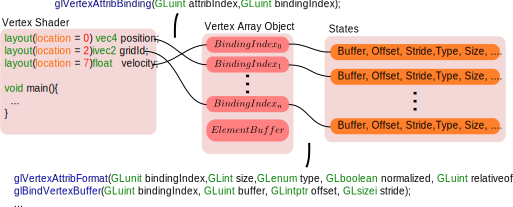
\includegraphics[width=11cm,keepaspectratio]{pics/vao.pdf}
  \end{figure}
\end{frame}

\begin{frame}[fragile]
\frametitle{VAO - příklad použití}
	Aplikace - inicializace
	{\scriptsize
	\begin{minted}[frame=lines]{c++}
	glGenVertexArrays(1,&VAO);//vygenerovani jmena VAO
	glBindVertexArray(VAO);//aktivovani VAO
	//nyni nastavime buffery a atributy
	glGenBuffers(1,&VBO);
	glBindBuffer(GL_ARRAY_BUFFER,VBO);
	glBufferData(GL_ARRAY_BUFFER,sizeof(Data),Data,GL_STATIC_DRAW);

	glGenBuffers(1,&EBO);
	glBindBuffer(GL_ELEMENT_ARRAY_BUFFER,EBO);
	glBufferData(GL_ELEMENT_ARRAY_BUFFER,sizeof(Index),Index,GL_STATIC_DRAW);

	glBindBuffer(GL_ARRAY_BUFFER,VBO);
	glEnableVertexAttribArray(vPos);
	glVertexAttribPointer(vPos,2,GL_FLOAT,GL_FALSE,sizeof(float)*5,
	  (GLvoid*)(sizeof(float)*0));

	glEnableVertexAttribArray(vCol);
	glVertexAttribPointer(vCol,3,GL_FLOAT,GL_FALSE,sizeof(float)*5,
	  (GLvoid*)(sizeof(float)*2));

	glBindVertexArray(0);//deaktivujeme VAO po tomto bode uz jej neovlivnujeme
	\end{minted}
	}
\end{frame}

\begin{frame}[fragile]
\frametitle{VAO - příklad použití}
	Aplikace - vykreslení
	{\scriptsize
	\begin{minted}[frame=lines]{c++}
	glBindVertexArray(VAO);//aktivujeme VAO
	glDrawElements(GL_TRIANGLES,6,GL_UNSIGNED_INT,NULL);
	glBindVertexArray(0);//deaktivujeme VAO
	\end{minted}
	}
\end{frame}


\bluepage{Advanced Draw Calls}

\begin{frame}[fragile]
\frametitle{Advanced draw commands}
	\begin{itemize}
	\item There is a lot of variants of following commands:
\begin{minted}[bgcolor=bg]{packages/c_cpp.py:CppLexer -x}
glDrawArrays glDrawElements
\end{minted}
	\item Instancing
	\item Indirect Draw
  \item Multi Draw
	\end{itemize}
{\tiny
\begin{minted}[bgcolor=bg]{packages/c_cpp.py:CppLexer -x}
glDrawArrays,glMultiDrawArrays

glDrawArraysInstanced,glDrawArraysInstancedBaseInstance,

glDrawArraysIndirect,glMultiDrawArraysIndirect

glDrawElements,glDrawRangeElements,glMultiDrawElements

glDrawElementsBaseVertex,glDrawRangeElementsBaseVertex,glMultiDrawElementsBaseVertex
glDrawElementsInstanced,glDrawElementsInstancedBaseInstance,glDrawElementsInstancedBaseVertex, 
glDrawElementsInstancedBaseVertexBaseInstance

glDrawElementsIndirect,glMultiDrawElementsIndirect
\end{minted}
}
\end{frame}

\begin{frame}[fragile]
\frametitle{Advanced draw commands - instancing}
	\begin{figure}[h]
	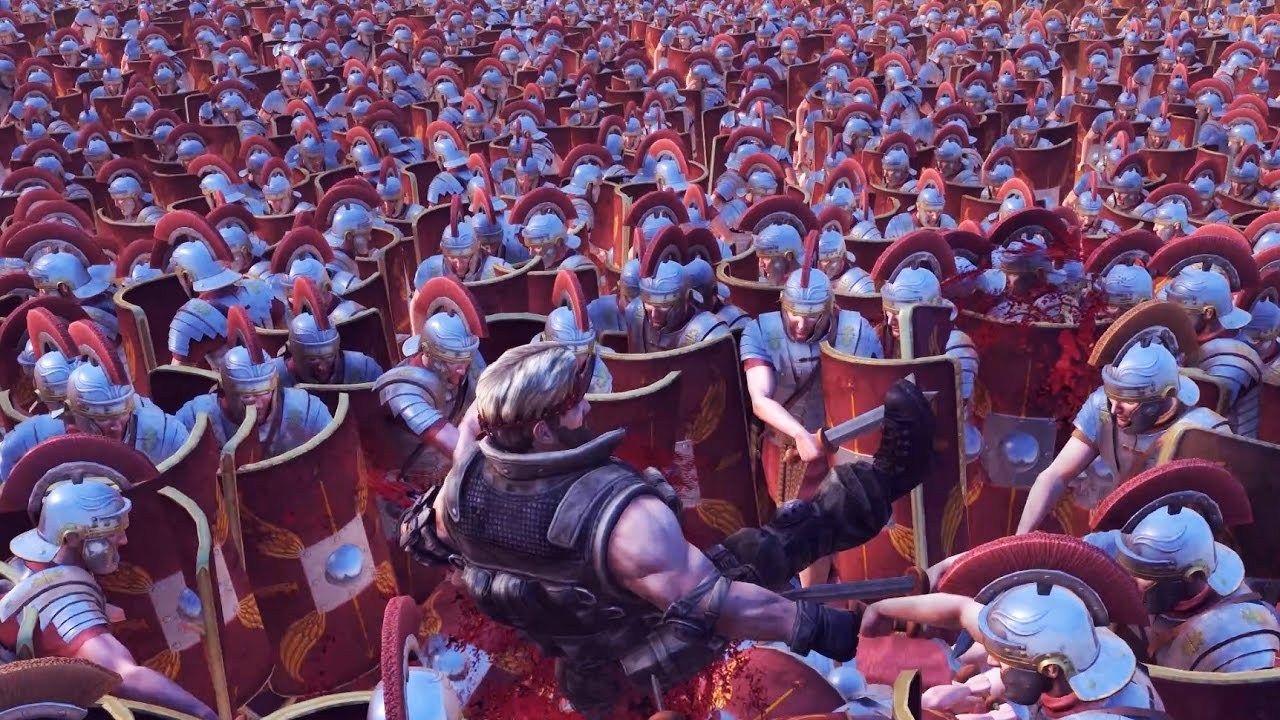
\includegraphics[width=10cm,keepaspectratio]{pics/uebs_instancing.jpg}
	\end{figure}
\url{http://epicbattles.wikia.com/wiki/File:UEBS_Chunk.jpg}
\end{frame}

\begin{frame}[fragile]
\frametitle{Advanced draw commands - instancing}
	\begin{itemize}
	\item Instancing draws same mesh in multiple instances, each with different transformation matrix.
	\item Instance id can be access in shader through built-in variable: gl\_InstanceID
	\item Instance id can be used as index into array of transformation matrices or materials.
	\end{itemize}
{\scriptsize
\begin{minted}[bgcolor=bg]{packages/graphics.py:GLShaderLexer -x}
#version 460

layout(location=0)in vec4 Position;
uniform mat4 MVP[100];

void main(){
  gl_Position=MVP[gl_InstanceID]*Position;
}
\end{minted}
}
{\scriptsize
\begin{minted}[bgcolor=bg]{packages/c_cpp.py:CppLexer -x}
glBindVertexArray(VAO);
glDrawArraysInstanced(GL_TRIANGLES,0,NumVertices,NumInstances);
glBindVertexArray(0);
\end{minted}
}
\end{frame}

\begin{frame}[fragile]
\frametitle{Advanced draw commands - indirect calls}
	\begin{figure}[h]
	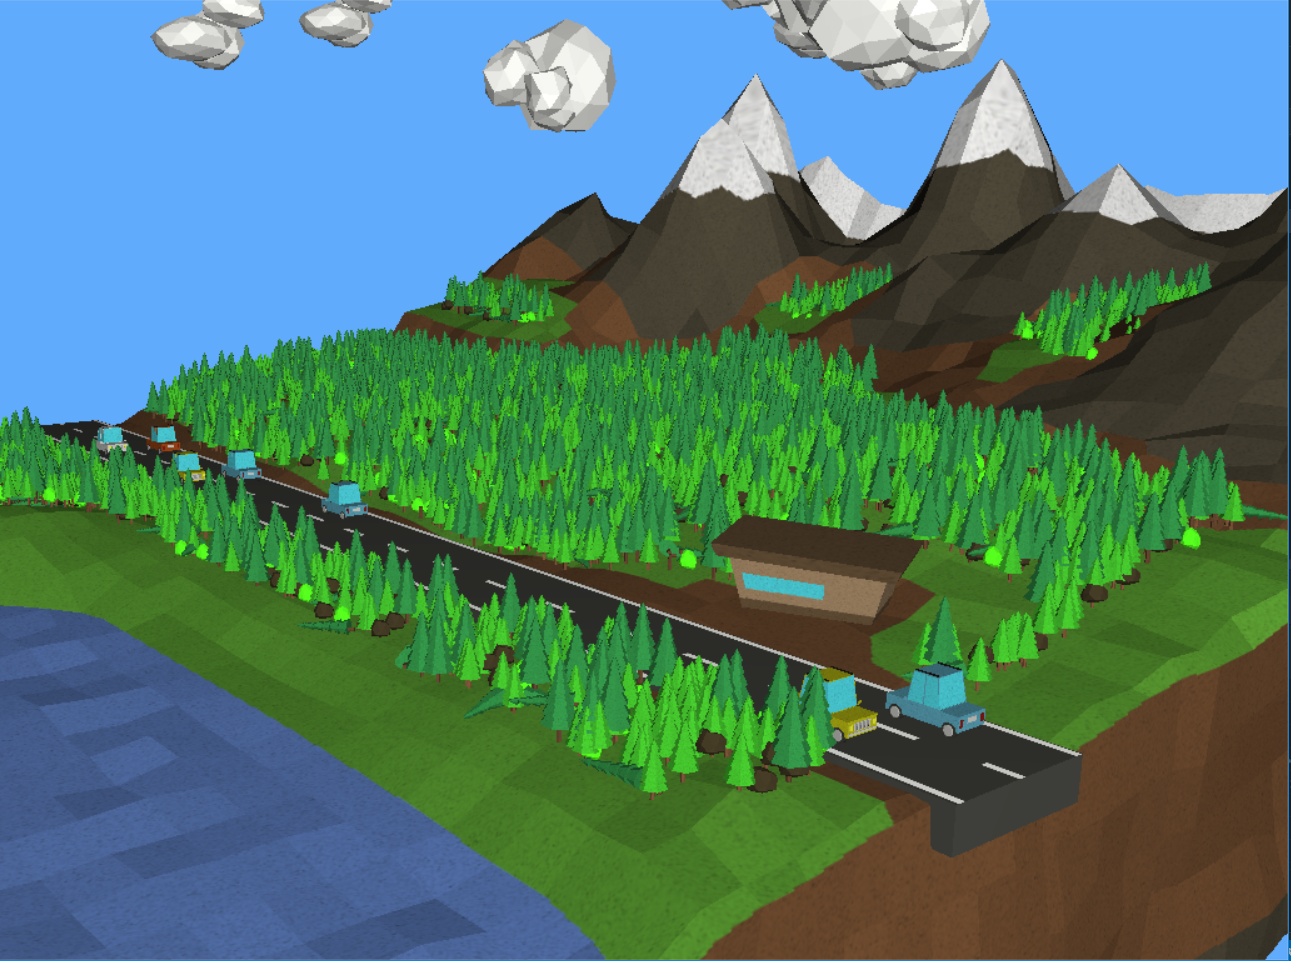
\includegraphics[width=10cm,keepaspectratio]{pics/indirect.png}
	\end{figure}
\url{http://www.fit.vutbr.cz/study/DP/DP.php.cs?id=18392&file=t}
\end{frame}

\begin{frame}[fragile]
\frametitle{Advanced draw commands - indirect draw calls}
	\begin{itemize}
  \item Draw call can be stored in buffers.
  \item There is no need for CPU synchronization.
  \item It can be combined with compute shader, atomic counters, transform feedback, ...
	\end{itemize}
{\scriptsize
\begin{minted}[bgcolor=bg]{packages/c_cpp.py:CppLexer -x}
//init
glGenBuffers(1,&IndirectBuffer);
glBindBuffer(GL_DRAW_INDIRECT_BUFFER,IndirectBuffer);
unsigned Data[4]={100,1,0,0};//command
glBufferData(GL_DRAW_INDIRECT_BUFFER,sizeof(unsigned)*4,
  Data,GL_DYNAMIC_DRAW);

//...
//fill buffer from GPU
//...

//draw
glBindBuffer(GL_DRAW_INDIRECT_BUFFER,IndirectBuffer);
glDrawArraysIndirect(GL_TRIANGLES,NULL);
\end{minted}
}
\end{frame}

\begin{frame}[fragile]
\frametitle{Advanced draw commands - multi draw calls}
	\begin{itemize}
    \item Multi draw call fuses a lot of single draw calls into one.
    \item All draw calls parameters can be stored in buffers and generated on GPU.
    \item Frustum Culling on GPU - number of instances of visible object objekt > 0
	\end{itemize}
{\scriptsize
\begin{minted}[bgcolor=bg]{packages/c_cpp.py:CppLexer -x}
//init
glGenBuffers(1,&IndirectBuffer);
glBindBuffer(GL_DRAW_INDIRECT_BUFFER,IndirectBuffer);
glBufferData(GL_DRAW_INDIRECT_BUFFER,sizeof(unsigned)*5*NumSpheres,
  NULL,GL_DYNAMIC_COPY);
//...
glDispatchCompute(NumSpheres/WorkGroupSize.x+1,1,1);
//...
//draw
glBindVertexArray(VAO);
glBindBuffer(GL_DRAW_INDIRECT_BUFFER,IndirectBuffer);
glMultiDrawElementsIndirect(GL_TRIANGLES,GL_UNSIGNED_INT,NULL,
  NumSpheres,sizeof(unsigned)*5);
glBindVertexArray(0);
\end{minted}
}
\end{frame}


\bluepage{Bindless textures}

\begin{frame}[fragile]
\frametitle{Bindless textures}
  \begin{itemize}
    \item We often need to draw a lot of objects with different textures.
    \item This leads to texture switching in between draw commands and to greater number of draw commands.
    \item Texture binding is not cheap and there is limited number of texture units.
    \item Texture atlas has its own problems (mipmapping, color bleeding, ...)
    \item There is an extension: \textcolor{blue}{ARB\_bindless\_texture} that solves a lot of problems
    \item This extension allows shader to switch textures directly.
    \item Textures are not explicitely bind to any texture unit.
  \end{itemize}
\end{frame}

\begin{frame}[fragile]
\frametitle{Bindless textures - handles}
{\scriptsize
\begin{minted}[bgcolor=bg]{packages/c_cpp.py:CppLexer -x}
#define MAX_TEXTURES 512
GLuint textures[MAX_TEXTURES];//list of textures
glCreateTextures(GL_TEXTURE_2D,MAX_TEXTURES,textures);//create textures
for(unsigned i=0;i<MAX_TEXTURES;++i){//loop over textures
  glTextureStorage2D(textures[i],1,GL_RGBA32F,1024,1024);//texture allocation
  glTextureSubImage2D(textures[i],0,0,0,1024,1024,
    GL_RGBA,GL_UNSIGNED_BYTE,data[i]);//data upload
  ...
  
}
\end{minted}
}
{\scriptsize
\begin{minted}[bgcolor=bg]{packages/c_cpp.py:CppLexer -x}
GLuint64 handles[MAX_TEXTURES];//list of handles to textures
for(unsigned i=0;i<MAX_TEXTURES;++i){
  handles[i]=glGetTextureHandleARB(textures[i]);
  glMakeTextureHandleResidentARB(handles[i]);
}
\end{minted}
}
{\scriptsize
\begin{minted}[bgcolor=bg]{packages/c_cpp.py:CppLexer -x}
glProgramUniformHandleui64vARB(
    programId,//program id
    uniformLocation,//location of uniform variable
    MAX_TEXTURES,//number of handles
    handles);//handles
\end{minted}
}
\end{frame}

\begin{frame}[fragile]
\frametitle{Bindless textures - vertex shader}
{\scriptsize
\begin{minted}[bgcolor=bg]{packages/graphics.py:GLShaderLexer -x}
#version 440 core

#extension GL_ARB_bindless_texture : require

#define MAX_TEXTURES 512

layout(bindless_sampler)uniform sampler2D textures[MAX_TEXTURES];
flat out sampler2D sampler;

struct Material{
  uint  textureId;
  vec3  color;
};

layout(std430,binding=0)buffer MaterialArray{Material materials[];};

layout(location=3) in uint materialID;

void main(){
  sampler = textures[materials[materialID]];
  gl_Position=...;
}
\end{minted}
}
\end{frame}

\begin{frame}[fragile]
\frametitle{Bindless textures - fragment shader}
{\scriptsize
\begin{minted}[bgcolor=bg]{packages/graphics.py:GLShaderLexer -x}
#version 440 core

#extension GL_ARB_bindless_texture : require

layout(location=0)out vec4 fColor;

flat in sampler2D sampler;

in vec2 vTexCoord;

void main(){
  fColor=texture(sampler,vTexCoord);
}
\end{minted}
}
\end{frame}


\begin{frame}[fragile]
\frametitle{Frame Buffer Object (FBO)}
  \begin{itemize}
    \item Obvykle se scéna renderuje do defaultního framebufferu obrazovky.
    \item Od verze OpenGL 3.3 je umožněno vytvoření vlastního framebufferu a vykreslovat scénu do něj.
    \item Framebuffer se skládá z několika 2D polí (hloubkový buffer, stencil buffer, několik barevných bufferů).
    \item{FBO umožňují renderování do textur.}
    \item{Umožňují renderovat uživatelské informace (normály, pozici, hloubku, ...) (Multiple Render Targets).}
    \item{Jsou základem pro různé grafické efekty např. vody, SSAO.}
    \item{Umožňují odložené stínování (deferred shading).}
    \item{Layered rendering}
  \end{itemize}
\end{frame}

\begin{frame}
\frametitle{Frame Buffer Object}
  \begin{figure}[h]
  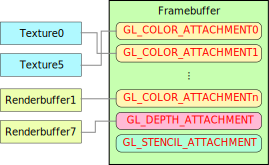
\includegraphics[width=10cm,keepaspectratio]{pics/framebuffer.pdf}
  \end{figure}
\end{frame}


\begin{frame}
\frametitle{Použití FBO}
    \begin{enumerate}
        \item{Získání jména FBO.}
        \item{Aktivování FBO.}
        \item{Připojení textur/renderbufferů k attachmentům.}
        \item{Nastavení seznamu attachmentů.}
        \item{Deaktivace FBO.}
        \item{...}
        \item{Aktivování FBO.}
        \item{Vykreslení scény.}
        \item{Deaktivace FBO.}
        \item{Zpracování vyrenderovaných textur.}
    \end{enumerate}
\end{frame}

\begin{frame}[fragile]
\frametitle{Vytvoření/uvolnění FBO identifikátorů}
  \begin{itemize}
    \item{
    Vytvoření VBO identifikátorů:
    {\scriptsize
    \mint[frame=lines]{c++}|void glGenFramebuffers(GLsizei n,GLuint * buffers);|
    }}
    \item{
    Uvolnění VBO identifikátorů:
    {\scriptsize
    \mint[frame=lines]{c++}|void glDeleteFramebuffers(GLsizei n,GLuint * buffers);|
    }}
  \end{itemize}
\end{frame}

\begin{frame}[fragile]
\frametitle{Ověření stavu FBO}
  \begin{itemize}
    \item{
    Pro ověření stavu FBO použijeme tuto funkci
    {\scriptsize
    \mint[frame=lines]{c++}|GLenum glCheckFramebufferStatus(GLenum target);|
    }}
    \item{
    Pokud funkce vraci {\color{red} GL\_FRAMEBUFFER\_COMPLETE} je vše v pořádku.
    }
  \end{itemize}
\end{frame}


\begin{frame}[fragile]
\frametitle{Aktivování/deaktivování FBO}
  \begin{itemize}
    \item{
    Aktivování/deaktivování FBO:
    {\scriptsize
    \mint[frame=lines]{c++}|void glBindFramebuffer(GLenum target,GLuint framebuffer);|
    }
    \begin{description}
    \item[target] GL\_FRAMEBUFFER stejný buffer pro čtení i zápis, GL\_READ\_FRAMEBUFFER, GL\_DRAW\_FRAMEBUFFER.
    \item[framebuffer] Jméno FBO získané {\color{blue} glGenFramebuffers}.
    Pokud nastaveno na 0 deaktivuje buffer.
    \end{description}
    }
  \end{itemize}
\end{frame}

\begin{frame}[fragile]
\frametitle{Připojení textur}
  \begin{itemize}
    \item{
    Attachment představuje jeden podbuffer FBO - například hloubkový buffer.
    Připojení textur k attachmentům:
    {\scriptsize
    \begin{minted}[frame=lines]{c++}
    void glFramebufferTexture2D(GLenum target,GLenum attachment,
      GLenum textarget,GLuint texture,GLint level);
    \end{minted}
    }
    \begin{description}
    \item[target] Stejné jako u {\color{blue} glBindFramebuffer}.
    \item[attachment] Které informace budeme zapisovat do textury.
    GL\_DEPTH\_ATTACHMENT - hloubkový buffer.
    GL\_STENCIL\_ATTACHMENT - stencil buffer.
    GL\_COLOR\_BUFFERx - barva, nebo jiná informace.
    Specifikováno pomocí fragment shaderu (layout).
    \item[textarget] GL\_TEXTURE\_2D nebo cube mapa.
    \item[texture] Identifikátor textury.
    \item[level] Stupeň mipmappingu.
    \end{description}
    }
  \end{itemize}
\end{frame}

\begin{frame}[fragile]
\frametitle{Nastavení seznamu attachmentů (MRT)}
  \begin{itemize}
    \item{
    Nastavením seznamu attachmentů definujeme, do kterých barevných bufferů se bude kreslit.
    {\scriptsize
    \begin{minted}[frame=lines]{c++}
    void glDrawBuffers(GLsizei n,const GLenum * bufs);
    \end{minted}
    }
    \begin{description}
    \item[n] Počet bufferů, do kterých budeme kreslit.
    \item[bufs] Seznam GL\_COLOR\_BUFFERx.
    Pořadí specifikuje, ke kterému layout ve fragment shaderu bude buffer navázán.
    \end{description}
    }
  \end{itemize}
\end{frame}

\begin{frame}[fragile]
\frametitle{Kompletní příklad}
    Do textur budeme vykreslovat barvu, normálu a hloubku.
    Fragment shader:
    {\scriptsize
    \begin{minted}[frame=lines]{glsl}
#version 430
layout(location=0)out vec4 fragColor;//jeden vystup - drawbuffer0
layout(location=1)out vec3 fragNormal;//druhy vystup - drawbuffer1
//...
void main(){
  //...
  fragColor=vec4(fCol,1);//zapis barvy
  fragNormal=(fNor+1)/2;//zapis normaly
}
    \end{minted}
    }
\end{frame}

\begin{frame}[fragile]
\frametitle{Kompletní příklad}
    Aplikace - inicializace:
    {\tiny
    \begin{minted}[frame=lines]{c++}
glTexImage2D(GL_TEXTURE_2D,0,GL_RGBA8F,WIDTH,HEIGHT,0,GL_RGBA,
  GL_UNSIGNED_BYTE,NULL);//alokujeme misto
//...
glTexImage2D(GL_TEXTURE_2D,0,GL_RGB32F,WIDTH,HEIGHT,0,GL_RGBA,
  GL_UNSIGNED_BYTE,NULL);//alokujeme misto
//...
glTexImage2D(GL_TEXTURE_2D,0,GL_DEPTH_COMPONENT24,
  WIDTH,HEIGHT,0,GL_DEPTH_COMPONENT,GL_UNSIGNED_BYTE,NULL);

glGenFramebuffers(1,&FBO);//vygenerujeme nazev pro FBO
glBindFramebuffer(GL_FRAMEBUFFER,FBO);

//navazani textur
glFramebufferTexture2D(GL_FRAMEBUFFER,GL_DEPTH_ATTACHMENT,
  GL_TEXTURE_2D,tDepth,0);//navazeme texturu pro hloubku
glFramebufferTexture2D(GL_FRAMEBUFFER,GL_COLOR_ATTACHMENT3,
  GL_TEXTURE_2D,tColor,0);//navazeme texturu pro barvu
glFramebufferTexture2D(GL_FRAMEBUFFER,GL_COLOR_ATTACHMENT5,
  GL_TEXTURE_2D,tNormal,0);//navazeme texturu pro normalu

GLenum drawBuffers[]={
  GL_COLOR_ATTACHMENT3,//layout(location=0)out vec4 fragColor;
  GL_COLOR_ATTACHMENT5//layout(location=1)out vec3 fragNormal;
};
glDrawBuffers(2,drawBuffers);//nastavime seznam cilu

if(glCheckFramebufferStatus(GL_FRAMEBUFFER)!=GL_FRAMEBUFFER_COMPLETE)
  std::cerr<<"chyba\n";
glBindFramebuffer(GL_FRAMEBUFFER,0);
    \end{minted}
    }
\end{frame}

\begin{frame}[fragile]
\frametitle{Kompletní příklad}
    Aplikace - kresleni:
    {\scriptsize
    \begin{minted}[frame=lines]{c++}
glBindFramebuffer(GL_FRAMEBUFFER,FBO);//aktivujeme FBO
glDrawArrays(...);
glBindFramebuffer(GL_FRAMEBUFFER,0);//deaktivovani FBO
    \end{minted}
    }
\end{frame}

\begin{frame}[fragile]
\frametitle{Kompletní příklad tvorba hier. z-bufferu}
		GLSL - CreateHierarchy:
		{\tiny
		\begin{minted}[frame=lines]{glsl}
		//vertex shader////////////////////////////////////////////////////////////
		#version 430
		void main(){
		  gl_Position=vec4(0);
		}
		//geometry shader//////////////////////////////////////////////////////////
		#version 430
		layout(points)in;
		layout(triangle_strip,max_vertices=4)out;
		void main(){
		  gl_Position=vec4(-1,-1,0,1);EmitVertex();
		  gl_Position=vec4(+1,-1,0,1);EmitVertex();
		  gl_Position=vec4(-1,+1,0,1);EmitVertex();
		  gl_Position=vec4(+1,+1,0,1);EmitVertex();
		}
		//fragment shader///////////////////////////////////////////////////////////
		#version 430
		layout(binding=0)uniform sampler2D Last;//last mipmap
		layout(location=0)out vec2 fDepth;//output depth
		ivec2 Coord=ivec2(gl_FragCoord.xy);//coordinates
		void main(void){
		  vec2 A=texelFetch(Last,Coord*2+ivec2(0,0),0).xy;
		  vec2 B=texelFetch(Last,Coord*2+ivec2(1,0),0).xy;
		  vec2 C=texelFetch(Last,Coord*2+ivec2(0,1),0).xy;
		  vec2 D=texelFetch(Last,Coord*2+ivec2(1,1),0).xy;
		  fDepth=vec2(min(min(A.x,B.x),min(C.x,D.x)),max(max(A.y,B.y),max(C.y,D.y)));
		}
		\end{minted}
		}
\end{frame}

\begin{frame}[fragile]
\frametitle{Kompletní příklad tvorba hier. z-bufferu}
		Aplikace - inicializace:
		{\scriptsize
		\begin{minted}[frame=lines]{c++}
		glGenTextures(1,&Depth);
		//textura obsahujici minimalni a maximalni hloubku
		glBindTexture(GL_TEXTURE_2D,Depth);
		glTexParameteri(GL_TEXTURE_2D,GL_TEXTURE_MAG_FILTER,GL_NEAREST);
		glTexParameteri(GL_TEXTURE_2D,GL_TEXTURE_MIN_FILTER,GL_NEAREST_MIPMAP_NEAREST);
		int Size=WSize;
		int Level=0;
		while(Size>0){//smycka pres levely
		  glTexImage2D(GL_TEXTURE_2D,Level++,GL_RG32F,Size,Size,0,GL_RG,
		    GL_FLOAT,NULL);//alokace vrstvy
		  Size/=2;
		}
		//render buffer s hloubkou
		glGenRenderbuffers(1,&RBO_Depth);
		glBindRenderbuffer(GL_RENDERBUFFER,RBO_Depth);
		glRenderbufferStorage(GL_RENDERBUFFER,GL_DEPTH_COMPONENT,WSize,WSize);

		glGenFramebuffers(1,&FBO);//vygenerujeme nazev pro FBO
		\end{minted}
		}
\end{frame}

\begin{frame}[fragile]
\frametitle{Kompletní příklad tvorba hier. z-bufferu}
		Aplikace - render2 - tvorba hierarchie:
		{\tiny
		\begin{minted}[frame=lines]{c++}
		glUseProgram(CreateHierarchy);
		int Level=1;
		int ActSize=WSize/2;
		glBindFramebuffer(GL_FRAMEBUFFER,HFBO);//bind framebuffer
		glActiveTexture(GL_TEXTURE0);//activate tex. unit 0
		glBindTexture(GL_TEXTURE_2D,Depth);//bind depth texture to tex. unit 0
		while(ActSize>0){//while there are
		  glViewport(0,0,ActSize,ActSize);//set viewport
		  glTexParameteri(GL_TEXTURE_2D,GL_TEXTURE_BASE_LEVEL,Level-1);//starting mipmap level
		  glTexParameteri(GL_TEXTURE_2D,GL_TEXTURE_MAX_LEVEL,Level-1);//max mipmap level
		  glFramebufferTexture2D(GL_FRAMEBUFFER,GL_COLOR_ATTACHMENT0,GL_TEXTURE_2D,Depth,Level);
		  GLenum DrawBuffers[]={GL_COLOR_ATTACHMENT0};
		  glDrawBuffers(1,DrawBuffers);
		  glDrawArrays(GL_POINTS,0,1);
		  Level++;//increment level of mipmap
		  ActSize/=2;//actual size of mipmap
		}
		glBindFramebuffer(GL_FRAMEBUFFER,0);//unbind framebffer
		glTexParameteri(GL_TEXTURE_2D, GL_TEXTURE_BASE_LEVEL, 0);//starting mipmap level
		glTexParameteri(GL_TEXTURE_2D, GL_TEXTURE_MAX_LEVEL, Level-1);//max mipmap level
		glViewport(0,0,WSize,WSize);//reset viewport
		\end{minted}
		}
\end{frame}



\bluepage{Direct State Access}

\begin{frame}[fragile]
\frametitle{Direct State Access}
	\begin{figure}[h]
	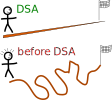
\includegraphics[width=8cm,keepaspectratio]{pics/dsa.pdf}
	\end{figure}
\end{frame}

\begin{frame}
  \frametitle{Direct State Access}
  \begin{itemize}
    \item Since OpenGL 4.5, Khronos added large extension into core profile - Direct State Access.
    \item DSA adds a lot of new functions for direct manipulation of objects.
    \item Bind to modify paradigm will be deprecated in the future.
  \end{itemize}
  Old approach:
  \begin{enumerate}
    \item Backup object id that is currently bound to target.
    \item Bind new object to target.
    \item Execute operation on target.
    \item Rebind backup to target.
  \end{enumerate}
  New approach:
  \begin{enumerate}
    \item Execute operation on object.
  \end{enumerate}
\end{frame}

\begin{frame}
  \frametitle{Direct State Access}
  \begin{itemize}
    \item DSA is easier and follow common sense.
    \item DSA does not break bindings.
    \item DSA is faster, less state switching.
    \item Target is replaced with object id in most OpenGL functions.
    \item DSA exists as extension for a long time - it is supported on all GPUs
  \end{itemize}
\end{frame}

\begin{frame}[fragile]
  \frametitle{Direct State Access - examples}
    Bind to modify:
{\scriptsize
\begin{minted}[bgcolor=bg]{packages/c_cpp.py:CppLexer -x}
GLint old;
glGenRenderbuffers(1,&RBO);
glGetIntegerv(GL_RENDERBUFFER_BINDING,&old);
glBindRenderbuffer(GL_RENDERBUFFER,RBO);
glRenderbufferStorage(GL_RENDERBUFFER,internalFormat,width,height);
glBindRenderbuffer(GL_RENDERBUFFER,old);
\end{minted}
}
    Direct state access:
{\scriptsize
\begin{minted}[bgcolor=bg]{packages/c_cpp.py:CppLexer -x}
glCreateRenderbuffers(1,&RBO);
glNamedRenderbufferStorage(RBO,internalFormat,width,height);
\end{minted}
}
\end{frame}

\begin{frame}[fragile]
  \frametitle{Direct State Access - examples}
    Bind to modify:
{\scriptsize
\begin{minted}[bgcolor=bg]{packages/c_cpp.py:CppLexer -x}
glBindFramebuffer(GL_READ_FRAMEBUFFER,fbo);
glBindFramebuffer(GL_DRAW_FRAMEBUFFER,0);
glBlitFramebuffer(0,0,width,height,0,0,width,height,
  GL_COLOR_BUFFER_BIT,GL_NEAREST);
\end{minted}
}
    Direct state access:
{\scriptsize
\begin{minted}[bgcolor=bg]{packages/c_cpp.py:CppLexer -x}
glBlitNamedFramebuffer(fbo,0,0,0,width,height,0,0,width,height,
  GL_COLOR_BUFFER_BIT,GL_NEAREST);
\end{minted}
}
\end{frame}

\begin{frame}[fragile]
  \frametitle{Direct State Access - confusion}
  \begin{itemize}
    \item Some OpenGL functions have 2 or even 3 alternative commands.
    \item A lot of functions are redundant.
    \item Confusion in texture, framebuffer, vao commands
  \end{itemize}
{\tiny
\begin{minted}[bgcolor=bg]{packages/c_cpp.py:CppLexer -x}
glFramebufferTexture
glFramebufferTexture1D;
glFramebufferTexture2D;
glFramebufferTexture3D;
glFramebufferTextureLayer;
glNamedFramebufferTexture;
glNamedFramebufferTextureLayer;
\end{minted}
}
{\tiny
\begin{minted}[bgcolor=bg]{packages/c_cpp.py:CppLexer -x}
glVertexArrayBindingDivisor
glVertexAttribDivisor
glVertexBindingDivisor
\end{minted}
}
{\tiny
\begin{minted}[bgcolor=bg]{packages/c_cpp.py:CppLexer -x}
glTexImage2D
glTexStorage2D
glTextureStorage2D
\end{minted}
}
\end{frame}


\bluepage{Functionality Switching}

\begin{frame}[fragile]
\frametitle{Program branching, functionality switching}
  \begin{itemize}
    \item Graphics application contains a lot of different effects (bump mapping, shadows, paralax mapping, ...)
    \item Different effects require different shaders.
    \item Functionality switching can be performed on different levels.
    \item Switching program path using uniform variable.
    \item Subroutines switching
    \item Shader program pipelines switching
    \item Shader program switching
  \end{itemize}
\end{frame}

\begin{frame}[fragile]
\frametitle{Functionality switching - uniformn variables}
  The fastest functionality switch can be performed directly inside shader.
  However, there is per-invocation overhead.
  For example, vertex shader has to evaluate condition for every vertex (thread divergence).
{\scriptsize
\begin{minted}[bgcolor=bg]{packages/graphics.py:GLShaderLexer -x}
#version 430
uniform uint method;
void main(){
  switch(method){
    case 1:
      normalMapping(...);
      break;
    case 2:
      paralaxMapping(...);
      break;
    case 3:
      ...
  }
}
\end{minted}
}
\end{frame}

\begin{frame}[fragile]
\frametitle{Functionality switching - subroutines}
  It is the second fastest functionality switch. It is function pointer switching.
{\tiny
\begin{minted}[bgcolor=bg]{packages/graphics.py:GLShaderLexer -x}
#version 440

layout(location=0)out vec4 fColor;

subroutine vec4 getColorSubroutine();
subroutine vec4 rotateColorSubroutine(vec4);

subroutine (getColorSubroutine) vec4 redColor(){return vec4(1,0,0,1);}
subroutine (getColorSubroutine) vec4 greenColor(){return vec4(0,1,0,1);}

subroutine (rotateColorSubroutine) vec4 rotate1Left (vec4 c){return c.yzwx;}
subroutine (rotateColorSubroutine) vec4 rotate2Left (vec4 c){return c.zwxy;}
subroutine (rotateColorSubroutine) vec4 rotate3Left (vec4 c){return c.wxyz;}
subroutine (rotateColorSubroutine) vec4 reverse     (vec4 c){return c.wzyx;}

subroutine uniform getColorSubroutine    getColor;//fce pointer
subroutine uniform rotateColorSubroutine rotateColor[3];//array of fce pointers

uniform uint rotateIndex=0;

void main(){
  fColor=rotateColor[rotateIndex](getColor());
}
\end{minted}
}
\end{frame}

\begin{frame}[fragile]
\frametitle{Functionality switching - subroutines}
{\tiny
\begin{minted}[bgcolor=bg]{packages/c_cpp.py:CppLexer -x}
//all subroutines
GLuint sl0=glGetSubroutineIndex(program,GL_FRAGMENT_SHADER,"redColor");
GLuint sl1=glGetSubroutineIndex(program,GL_FRAGMENT_SHADER,"greenColor");
GLuint sl2=glGetSubroutineIndex(program,GL_FRAGMENT_SHADER,"rotate1Left");
GLuint sl3=glGetSubroutineIndex(program,GL_FRAGMENT_SHADER,"rotate2Left");
GLuint sl4=glGetSubroutineIndex(program,GL_FRAGMENT_SHADER,"rotate3Left");
GLuint sl5=glGetSubroutineIndex(program,GL_FRAGMENT_SHADER,"reverse");

//uniform offsets for subroutines
GLuint sul0=glGetSubroutineUniformLocation(program,GL_FRAGMENT_SHADER,"getColor");
GLuint sul1=glGetSubroutineUniformLocation(program,GL_FRAGMENT_SHADER,"rotateColor");

glUseProgram(program);
//list of all slots for subroutines
GLuint sl[4];
sl[sul0+0]=sl1;
sl[sul1+0]=sl5;
sl[sul1+1]=sl2;
sl[sul1+2]=sl3;
glUniformSubroutinesuiv(GL_FRAGMENT_SHADER,4,sl);
\end{minted}
}
\end{frame}

\begin{frame}[fragile]
\frametitle{Functionality switching - pipelines}
\begin{itemize}
  \item Program pipelines can be used for shader stage switching (vertex,fragment,geometry,...).
  \item Inputs and outputs of stages has to match, they will not be checked.
  \item Pipeline switching is cheaper that program switching.
  \item It is usefull in situation where there is a lot of similar shader programs.
\end{itemize}
{\tiny
\begin{minted}[bgcolor=bg]{packages/c_cpp.py:CppLexer -x}
GLuint vs,gs,fs;
//This function creates shader program that contains only one shader stage.
vs=glCreateShaderProgramv(GL_VERTEX_SHADER,1,&vstext);
fs=glCreateShaderProgramv(GL_FRAGMENT_SHADER,1,&fstext);
//...

GLuint pipeline;
glGenPipelines(1,&pipeline);
glBindPipelines(pipeline);

//...
glUseProgramStages(pipeline,GL_VERTEX_SHADER_BIT,vs);
glUseProgramStages(pipeline,GL_GEOMETRY_SHADER_BIT,program);//select geometry shader from shader program
glUseProgramStages(pipeline,GL_FRAGMENT_SHADER_BIT,fs);
\end{minted}
}
\end{frame}


\bluepage{Geometry Shaders}

\begin{frame}[fragile]
\frametitle{Geometry shader}
	\begin{itemize}
  \item Geometry shader is located after vertex shader (after tessellation).
	\item Geometry shader is executed per primitive - it has access to all vertices of a primitive.
	\item It can generate new geometry or modify current geometry.
  \item It can transform point into quad (usefull for particle simulation).
  \item It can be used for several effects (shadow volumes, particle systems, ...).
	\item Geometry Instancing.
	\item Transform feedback.
	\end{itemize}
\end{frame}

\begin{frame}[fragile]
\frametitle{Geometry shader - inputs/outputs}
	\begin{itemize}
	\item Type of inputs and outputs has to be specified inside geometry shader.
{\scriptsize
\begin{minted}[bgcolor=bg]{packages/graphics.py:GLShaderLexer -x}
layout(points,invocations=N)in;//input primitive will be point.
//points, lines, lines_adjacency, triangles, triangles_adjacency
//geometry shader will be executed N times on each point.
\end{minted}
}
	\item Type of output primitive and number of output vertices has to be specified.
{\scriptsize
\begin{minted}[bgcolor=bg]{packages/graphics.py:GLShaderLexer -x}
layout(triangle_strip,max_vertices=4)out;//output primitive and max number of vertices
//points, line_strip, triangle_strip
\end{minted}
}
	\end{itemize}
\end{frame}

\begin{frame}[fragile]
\frametitle{Geometry shader - point to quad}
	\begin{figure}[h]
		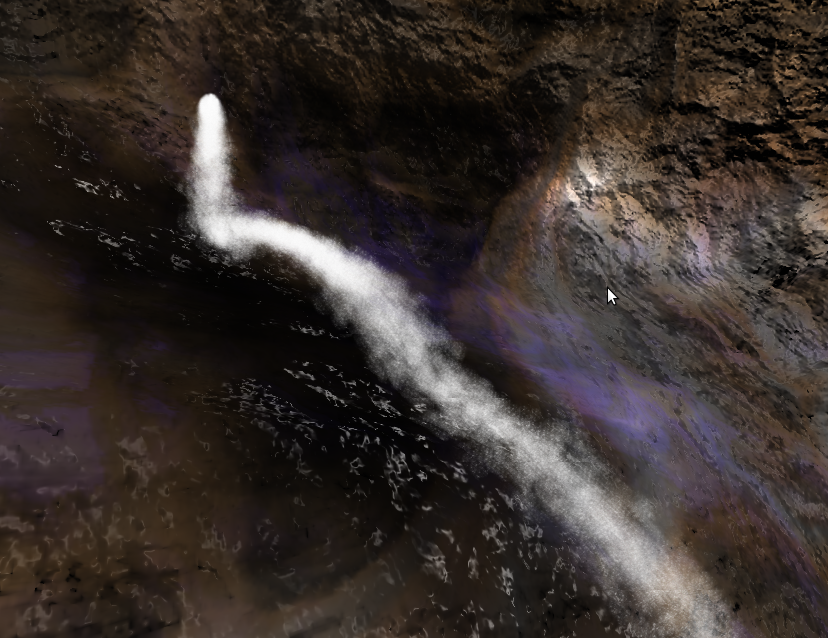
\includegraphics[width=9cm,keepaspectratio]{pics/gs.pdf}
	\end{figure}

{\scriptsize
\begin{minted}[bgcolor=bg]{packages/graphics.py:GLShaderLexer -x}
#version 430

layout(points)in;
layout(triangle_strip,max_vertices=4)out;

void main(){
  gl_Position=mvp*(gl_in[0].gl_Position+vec4(-1,-1,0,0));
  EmitVertex();
  gl_Position=mvp*(gl_in[0].gl_Position+vec4(-1,+1,0,0));
  EmitVertex();
  gl_Position=mvp*(gl_in[0].gl_Position+vec4(+1,-1,0,0));
  EmitVertex();
  gl_Position=mvp*(gl_in[0].gl_Position+vec4(+1,+1,0,0));
  EmitVertex();
  EndPrimitive();
}
\end{minted}
}
\end{frame}

\begin{frame}[fragile]
\frametitle{Geometry shader - fullscreen quad}
{\scriptsize
\begin{minted}[bgcolor=bg]{packages/graphics.py:GLShaderLexer -x}
#version 430
layout(points)in;
layout(triangle_strip,max_vertices=4)out;
void main(){
  gl_Position=vec4(-1,-1,0,1);EmitVertex();
  gl_Position=vec4(-1,+1,0,1);EmitVertex();
  gl_Position=vec4(+1,-1,0,1);EmitVertex();
  gl_Position=vec4(+1,+1,0,1);EmitVertex();
  EndPrimitive();
}
\end{minted}
}
{\scriptsize
\begin{minted}[bgcolor=bg]{packages/c_cpp.py:CppLexer -x}
glGenVertexArrays(1,&emptyVAO);
//...
glBindVertexArray(emptyVAO);//activate VAO
glDrawArrays(GL_POINTS,0,1);
glBindVertexArray(0);//deactivate VAO
\end{minted}
}
\end{frame}

\begin{frame}[fragile]
\frametitle{Shadow volumes - zfail}
  \begin{figure}[h]
    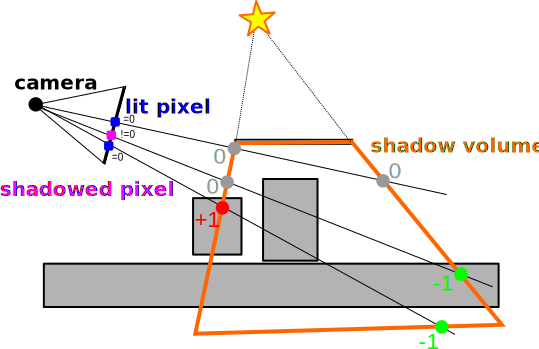
\includegraphics[width=11cm,keepaspectratio]{pics/shadowvolume.pdf}
  \end{figure}
\end{frame}

\begin{frame}[fragile]
\frametitle{Geometry shader - Shadow volumes}
  \begin{columns}[T]
    \begin{column}{.44\textwidth}
{\tiny
\begin{minted}[bgcolor=bg]{packages/graphics.py:GLShaderLexer -x}
#version 330
layout(triangles)in;
layout(triangle_strip,max_vertices=10)out;
uniform mat4 MVP,M;//matrices
uniform vec4 LightPosition;//light position
void main(){
  vec4 LP=M*LightPosition;
  vec4 p[6];
  p[0]=gl_in[0].gl_Position;//triangle vertices
  p[1]=gl_in[1].gl_Position;
  p[2]=gl_in[2].gl_Position;
  //triangle points projected to infinity
  p[3]=vec4(gl_in[0].gl_Position.xyz*LP.w-LP.xyz,0);
  p[4]=vec4(gl_in[1].gl_Position.xyz*LP.w-LP.xyz,0);
  p[5]=vec4(gl_in[2].gl_Position.xyz*LP.w-LP.xyz,0);
  vec3 N=normalize(cross((p[1]-p[0]).xyz,(p[2]-p[0]).xyz));
  float Distance=dot(N,LP.xyz)-dot(N,p[0].xyz);
  if(Distance<=0){//flip volume inside out
    vec4 c=p[0];p[0]=p[1];p[1]=c;
    c=p[3];p[3]=p[4];p[4]=c;
  }
  gl_Position=MVP*p[0];EmitVertex();
  gl_Position=MVP*p[1];EmitVertex();
  gl_Position=MVP*p[3];EmitVertex();
  gl_Position=MVP*p[4];EmitVertex();
  gl_Position=MVP*p[5];EmitVertex();
  gl_Position=MVP*p[1];EmitVertex();
  gl_Position=MVP*p[2];EmitVertex();
  gl_Position=MVP*p[0];EmitVertex();
  gl_Position=MVP*p[5];EmitVertex();
  gl_Position=MVP*p[3];EmitVertex();
  EndPrimitive();
}
\end{minted}
}
    \end{column}
    \begin{column}{.48\textwidth}
	    \begin{figure}[h]
    		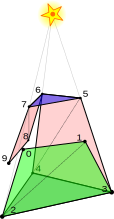
\includegraphics[width=3cm,keepaspectratio]{pics/PerTriangle.pdf}
    	\end{figure}
    \end{column}
  \end{columns}

\end{frame}


\begin{frame}
\frametitle{Transform feedback}
	\begin{itemize}
  \item Transform feedback stops rendering pipeline before rasterisation and sends primitives into buffers.
	\item It can be used in vertex shader and geometry shader.
  \item It can be combined with rendering (streams).
	\end{itemize}
	\begin{figure}[h]
	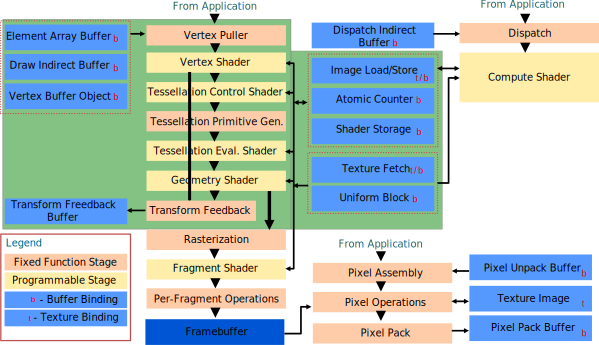
\includegraphics[width=10cm,keepaspectratio]{pics/tf_pipeline}
	\end{figure}
\end{frame}

\begin{frame}
\frametitle{Transform feedback}
	\begin{figure}[h]
	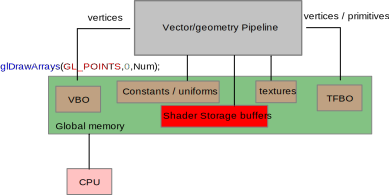
\includegraphics[width=10cm,keepaspectratio]{pics/tf_mem}
	\end{figure}
\end{frame}

\begin{frame}[fragile]
\frametitle{Transform feedback - example}
	{\scriptsize
	\begin{minted}[frame=lines]{c++}
const char*Vayrings[]={"Out1", "Out2"};
glTransformFeedbackVaryings(Program,2,Varyings,GL_SEPARATE_ATTRIBS);
glLinkProgram(Program);

//...

glBindBufferBase(GL_TRANSFORM_FEEDBACK_BUFFER,0,Buffer1);
glBindBufferBase(GL_TRANSFORM_FEEDBACK_BUFFER,1,Buffer2);

glEnable(GL_RASTERIZER_DISCARD);//nebudeme rasterizovat
//...
glBeginTransformFeedback(GL_TRIANGLES);
glDrawArrays(...);
glEndTransformFeedback();
	\end{minted}
	}
\end{frame}

\begin{frame}[fragile]
\frametitle{Transform Feedback - Inicialization}
  We have to link shader program with marked varyings.
	c++:
	{\scriptsize
	\begin{minted}[frame=lines]{cpp}
//list of variables that will be written into buffer(s).
const char*ResetVaryings[]={"vPosition","vVelocity","vMass"};
//set varyings and interleaving
glTransformFeedbackVaryings(ResetProgram,3,ResetVaryings,GL_INTERLEAVED_ATTRIBS);
//relink shader program
glLinkProgram(ResetProgram);
	\end{minted}
	}
	glsl:
	{\scriptsize
	\begin{minted}[frame=lines]{glsl}
#version 330

layout(location=0)out vec2  vPosition;//particle position
layout(location=1)out vec2  vVelocity;//particle velocity
layout(location=2)out float vMass;//particle mass
//...
void main(){
  vPosition = vec2(0);//init position
  vVelocity = vec2(cos(VelAngle),sin(VelAngle))*VelSize;//init velocity
  vMass     = Noise(MassSeed+uint(gl_VertexID),MinMass,MaxMass);//init mass
}
	\end{minted}
	}
\end{frame}


\begin{frame}[fragile]
\frametitle{OpenGL tessellation}
	\begin{itemize}
	\item Tessellation splits one primitive into more joint sub primitives.
	\item It can be used to refine details of a geometry.
	\item Tessellation is located between vertex shader and geometry shader.
	\item It is composed of three parts:
	\begin{itemize}
	\item Control Shader
	\item Primitive generation/tessellation
	\item Evaluation Shader
	\end{itemize}
	\item There is one new primitive type - \textcolor{red}{GL\_PATCHES}
	\end{itemize}
  {\scriptsize
	\begin{minted}[frame=lines]{c++}
glPatchParameteri(GL_PATCH_VERTICES,10);//set number of vertices of patch to 10
glDrawArrays(GL_PATCHES,0,200);//draw 20 patches (each is composed of 10 vertices)
	\end{minted}
  }
	\begin{figure}[h]
	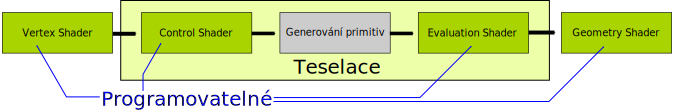
\includegraphics[width=10cm,keepaspectratio]{pics/tess_pipeline.pdf}
	\end{figure}
\end{frame}

\begin{frame}
\frametitle{Control Shader}
	\begin{itemize}
	\item CS controls level of tessellation.
	\item It computes control vertices.
	\item CS is invocated as many times as there is output vertices in output patch primitive.
	\item A invocation number is stored in built-in variable \textcolor{OliveGreen}{gl\_InvocationID}.
	\item We can synchronise threads in CS using \textcolor{OliveGreen}{barrier}().
	\end{itemize}
	\begin{figure}[h]
	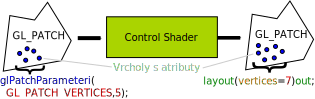
\includegraphics[width=10cm,keepaspectratio]{pics/tess_control.pdf}
	\end{figure}
\end{frame}

\begin{frame}
    \frametitle{Parameters}

    \includegraphics[width=\textwidth]{pics/tess.pdf}

    \begin{itemize}
				\item \textcolor{OliveGreen}{layout}
					(\{\textcolor{orange}{isolines},\textcolor{orange}{triangles},\textcolor{orange}{quads}\})
					\textcolor{OliveGreen}{in};
				\item \textcolor{OliveGreen}{gl\_TessLevelOuter}[4],\textcolor{OliveGreen}{gl\_TessLevelInner}[2]
    \end{itemize}
\end{frame}

\begin{frame}[fragile]
\frametitle{Control Shader - example}
	{\scriptsize
	\begin{minted}[frame=lines]{glsl}
#version 430

// number of output vertices in output patch primitive ==
// number of threads per patch primitive
layout(vertices=3)out;

uniform vec2 TessLevelInner;//there are two inner and
uniform vec4 TessLevelOuter;//four outer levels of tessellation

void main(){
  //number of elements in gl_in depends on GL_PATCH_VERTICES
  //number of elements in gl_out delends on layout(vertices=n)out;
  //In this case, number of elements in gl_in and gl_out is the same.
  gl_out[gl_InvocationID].gl_Position=gl_in[gl_InvocationID].gl_Position;//copy
  if(gl_InvocationID==0){//the first thread sets tessellation levels
    gl_TessLevelOuter[0]=TessLevelOuter[0];
    gl_TessLevelOuter[1]=TessLevelOuter[1];
    gl_TessLevelOuter[2]=TessLevelOuter[2];
    gl_TessLevelOuter[3]=TessLevelOuter[3];
    gl_TessLevelInner[0]=TessLevelInner[0];
    gl_TessLevelInner[1]=TessLevelInner[1];
  }
}
	\end{minted}
	}
\end{frame}

\begin{frame}
\frametitle{Evaluation Shader}
	\begin{itemize}
		\item It sets type of tessellated primitive: \textcolor{Orange}{isolines},\textcolor{orange}{triangles},\textcolor{orange}{quads}
		\item It computes coordinates of tessellated vertices.
		\item \textcolor{OliveGreen}{gl\_TessCoord} variable holds barycentric, uv, or normalized coords of tessellated vertices inside of primitive.
		\item Evaluation shader is executed for every tessellated vertex.
		\item Tessellated primiteves continue their path to geometry shader.
	\end{itemize}
	\begin{figure}[h]
	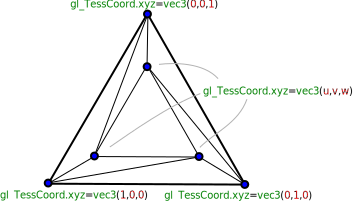
\includegraphics[width=7cm,keepaspectratio]{pics/tess_coord.pdf}
	\end{figure}
\end{frame}


\begin{frame}[fragile]
\frametitle{Evaluation Shader - example}
	\begin{itemize}
		\item Tessellated quad
		\item Computation of coordinates of tessellated vertices
	\end{itemize}
	{\scriptsize
	\begin{minted}[frame=lines]{glsl}
#version 430

layout(quads)in;

void main(){
  vec4 A=mix(gl_in[0].gl_Position,gl_in[1].gl_Position,gl_TessCoord.x);
  vec4 B=mix(gl_in[3].gl_Position,gl_in[2].gl_Position,gl_TessCoord.x);
  gl_Position=mix(A,B,gl_TessCoord.y);
}
	\end{minted}
	}
\end{frame}


\begin{frame}[fragile]
  \frametitle{Béziér surface - example}
	{\scriptsize
	\begin{minted}[frame=lines]{glsl}
// Vertex shader	
#version 430
void main() {
  gl_Position = mvp*position;
}

// Control shader
#version 430
layout(vertices=16) out;

void main() {
  gl_out[gl_InvocationID].gl_Position =
  gl_in[gl_InvocationID].gl_Position;
  if(gl_InvocationID == 0) {
    gl_TessLevelInner[0] = gl_TessLevelInner[1] = 
    gl_TessLevelOuter[0] = gl_TessLevelOuter[1] =
    gl_TessLevelOuter[2] = gl_TessLevelOuter[3] = 64;
  }
}
\end{minted}
	}
\end{frame}

\begin{frame}[fragile]
    \frametitle{Béziér surface - example}
  	{\scriptsize
		\begin{minted}[frame=lines]{glsl}
// Evaluation shader
#version 430
layout(quads, ccw) in;

vec4 bernstein(float t) {
  return vec4((1-t)*(1-t)*(1-t), 3*t*(1-t)*(1-t), 3*t*t*(1-t), t*t*t);
}

void main() {
  vec4 bu = bernstein(gl_TessCoord.x);
  vec4 bv = bernstein(gl_TessCoord.y);
  vec4 position = vec4(0, 0, 0, 0);
  for(int y = 0; y < 4; ++y){
    for(int x = 0; x < 4; ++x){
      position += bu[x]*bv[y]*gl_in[4*y + x].gl_Position;
    }
  }
  gl_Position = position;
}
  	\end{minted}
		}
\end{frame}

\begin{frame}[fragile]
\frametitle{Communication between shader stages}
	{\tiny
	\begin{minted}[frame=lines]{glsl}
#version 430

//output vertex shader attributes
out vec4 vAttrib;
gl_Position

//intput control shader attributes
in  vec4 vAttrib[];//attribute from vertex shader, size == GL_PATCH_VERTICES
gl_in[].gl_Position;//a possition attribute from vertex shader

//output control shader attributes
out vec4 cAttrib[];//size == layout(vertices=size)out
patch out mat4 cM;//once per output patch primitive

//input evaluation shader attributes
in vec4 cAttrib[];//size == layout(vertices=size)out
patch in  mat4 cM;//once per input patch

//output evaluation shader attributes
out vec3 eNormal;

//input geometry shader attributes
in vec3 eNormal[];//size == 2 for line, size == 3 for triangle, ...
	\end{minted}
	}
\end{frame}

\begin{frame}[fragile]
    \frametitle{Example - replace triangles with circles}
  \begin{columns}[T]
    \begin{column}{.44\textwidth}
	    \begin{figure}[h]
    		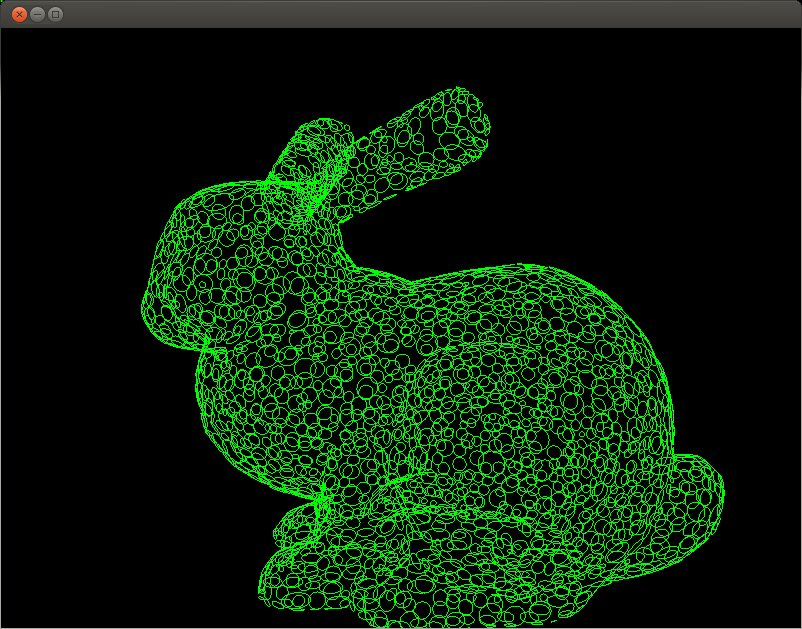
\includegraphics[width=5cm,keepaspectratio]{pics/ts_circle}
    	\end{figure}
    \end{column}
    \begin{column}{.48\textwidth}
 	    \begin{figure}[h]
    		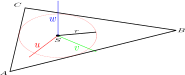
\includegraphics[width=5cm,keepaspectratio]{pics/circle.pdf}
    	\end{figure}
{\tiny
$$
K=
\left( 
\begin{array}{cccc} 
1 & 0 & 0 & S_x \\
0 & 1 & 0 & S_y \\
0 & 0 & 1 & S_z \\
0 & 0 & 0 & 1  \\
\end{array}
\right)
\cdot
\left( 
\begin{array}{cccc} 
r & 0 & 0 & 0 \\
0 & r & 0 & 0 \\
0 & 0 & r & 0 \\
0 & 0 & 0 & 1  \\
\end{array}
\right)
\cdot$$
$$
\left( 
\begin{array}{cccc} 
u_x & v_x & w_x & 0 \\
u_y & v_y & w_y & 0 \\
u_z & v_z & w_z & 0 \\
0 & 0 & 0 & 1  \\
\end{array}
\right)
$$
}
    \end{column}
  \end{columns}
\end{frame}

\begin{frame}[fragile]
    \frametitle{Example - replace triangles with circles}
  \begin{columns}[T]
    \begin{column}{.44\textwidth}
      Control Shader
  	{\tiny
		\begin{minted}[frame=lines]{glsl}
#version 400
layout(vertices=1)out;
patch out mat4 K;
void main(){
  gl_TessLevelOuter[0]=1;
  gl_TessLevelOuter[1]=64;
  gl_TessLevelOuter[2]=1;
  gl_TessLevelOuter[3]=1;
  gl_TessLevelInner[0]=1;
  gl_TessLevelInner[1]=1;
  vec4 TT[3];
  TT[0]=gl_in[0].gl_Position;
  TT[1]=gl_in[1].gl_Position;
  TT[2]=gl_in[2].gl_Position;
  float t01=length((TT[0]-TT[1]).xyz);
  float t02=length((TT[0]-TT[2]).xyz);
  float t12=length((TT[1]-TT[2]).xyz);
  float s=t01+t02+t12;
  float r=sqrt((s/2-t01)*(s/2-t02)*(s/2-t12)*s/2)*2/s;
  t01/=s;
  t02/=s;
  t12/=s;
  vec3 C=TT[0].xyz*t12+TT[1].xyz*t02+TT[2].xyz*t01;
  vec3 x=normalize(TT[0].xyz-C);
  vec3 y=normalize(TT[1].xyz-C);
  vec3 z=normalize(cross(x,y));
  y=normalize(cross(z,x));
  K=mat4(vec4(x,0)*r,vec4(y,0)*r,vec4(z,0)*r,vec4(C,1));
}
  	\end{minted}
		}
    \end{column}
    \begin{column}{.48\textwidth}
      Evaluation Shader
  	{\tiny
		\begin{minted}[frame=lines]{glsl}
#version 400

#define MY_PI 3.14159265359

layout(isolines)in;

uniform mat4 V;
uniform mat4 P;

patch in mat4 K;

void main(){
  float Angle=gl_TessCoord.x*MY_PI*2;
  vec4 PP=vec4(cos(Angle),sin(Angle),0,1);
  gl_Position=P*V*K*PP;
}
  	\end{minted}
		}
    \end{column}
  \end{columns}

\end{frame}


\begin{frame}
\frametitle{How to choose tessellation levels?}
	Outer level:
	\begin{itemize}
	\item Outer levels of edges of neighbor faces should be the same to prevent T-joints.
  \item Transform control points to the screen (screen-space distances).
	\item Divide edge length by maximal edge length.
	\end{itemize}
	Inner level:
	\begin{itemize}
	\item Average/maximum of outer levels
  \item ...
	\end{itemize}
\end{frame}


\begin{frame}
\frametitle{Image Load/Store}
	\begin{itemize}
	\item Reads/Writes from/to images inside of shader stage.
	\item There is new data type - image.
  \item An image is one layer of texture (one layer of mipmap, ...).
	\item There are atomic operation for images.
  \item Atomic operation are supported only for certain internal formats (integer, one channel).
  \item Image units (lequal 8 units) - simillar to texture units ( gequal 80 units).
	\item Store operations are side effect. They disable early fragment tests in fragment shader - it can be reenabled.
	\end{itemize}
\end{frame}

\begin{frame}
\frametitle{Image Load/Store}
	\begin{figure}[h]
	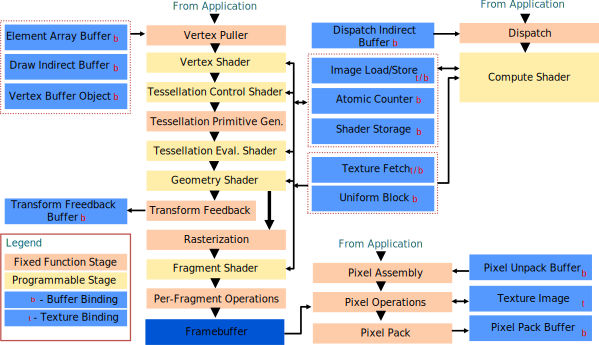
\includegraphics[width=11cm,keepaspectratio]{pics/opengl43.pdf}
	\end{figure}
\end{frame}

\begin{frame}[fragile]
\frametitle{Image Load/Store - example}
  This fragment shader emulates stencil buffer:
	{\scriptsize
	\begin{minted}[frame=lines]{glsl}
#version 430

layout(location=0)out vec4 fColor;
layout(early_fragment_tests)in;//enable early fragment tests
layout(r32i,location=0)uniform iimage2D myStencil;//integer image
ivec2 Coord=ivec2(gl_FragCoord.xy);//coordinates

void main(){
  if(gl_FrontFacing)//front face
    imageAtomicAdd(myStencil,Coord,+1);
  else
    imageAtomicAdd(myStencil,Coord,-1);
}
	\end{minted}
	}
\end{frame}

\begin{frame}[fragile]
\frametitle{Image Load/Store - example}
	{\scriptsize
	\begin{minted}[frame=lines]{c++}
//integer texture
glGenTextures(1,&Image);
glBindTexture(GL_TEXTURE_2D,Image);
glTexParameteri(GL_TEXTURE_2D,GL_TEXTURE_MAG_FILTER,GL_NEAREST);
glTexParameteri(GL_TEXTURE_2D,GL_TEXTURE_MIN_FILTER,GL_NEAREST);
glTexImage2D(GL_TEXTURE_2D,0,GL_R32I,Widht,Height,0,GL_RED_INTEGER,
  GL_UNSIGNED_BYTE,NULL);

//bind one layer of the texture onto zeroth image unit
glBindImageTexture(0,Image,0,GL_FALSE,0,GL_READ_WRITE,GL_R32I);

  \end{minted}
	}
\end{frame}


\bluepage{Atomic counters, Shader Storage Buffers}

\begin{frame}
\frametitle{Atomic counters/Shader Storage}
	Atomic counter:
	\begin{itemize}
	\item Atomic increment/decrement.
	\item It can be useds as index into shader storage buffers.
	\item Indirect Draw
	\end{itemize}
	Shader Storage Buffer
	\begin{itemize}
	\item Random access memory for shaders
	\item Atomic operation
	\item Binding points
	\end{itemize}
\end{frame}

\begin{frame}
\frametitle{Atomic counters/Shader Storage}
	\begin{figure}[h]
	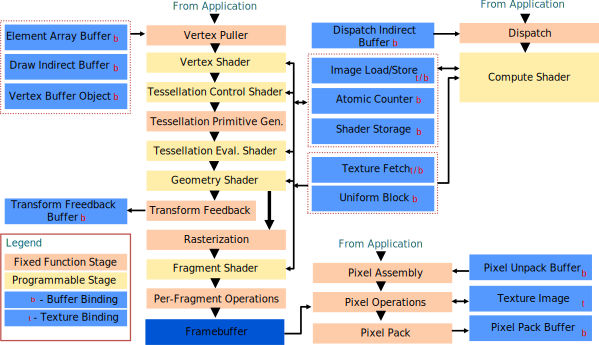
\includegraphics[width=11cm,keepaspectratio]{pics/opengl43.pdf}
	\end{figure}
\end{frame}

\begin{frame}[fragile]
\frametitle{Atomic counters/Shader Storage - example}
{\scriptsize
\begin{minted}[bgcolor=bg]{packages/graphics.py:GLShaderLexer -x}
#version 430

in vec4 vPos;

layout(binding=1,offset=0)uniform atomic_uint counter;
layout(std430,binding=0)buffer Output{vec4 data[];};

layout(location=0)vec4 fColor;
//...
void main(){
  int W=atomicCounterIncrement(counter);//increment counter
  data[w*2+0]=ComputeColor(...);//compute color
  data[w*2+1]=vPos;//write position
  //...
}
\end{minted}
}
\end{frame}

\begin{frame}[fragile]
\frametitle{Atomic counters/Shader Storage - example}
{\scriptsize
\begin{minted}[bgcolor=bg]{packages/c_cpp.py:CppLexer -x}
unsigned data[4]={0,0,0,0};
GLuint ACB;//identifier of a. counter
glCreateBuffers(1,&ACB);//create a. counter buffer
glNamedBufferData(ACB,sizeof(uint32_t)*4,data,GL_DYNAMIC_DRAW);
glBindBufferBase(GL_ATOMIC_COUNTER_BUFFER,1,ACB);//binding point 1

GLuint SSBO;//identifier of shader storage buffer
glCreateBuffers(1,&SSBO);//reserve identifier
glNamedBufferData(GL_SHADER_STORAGE_BUFFER,sizeof(float)*4*2*Max,
  NULL,GL_DYNAMIC_DRAW);
glClearNamedBufferData(SSBO,GL_R32F,GL_RED,GL_FLOAT,NULL);
glBindBufferRange(GL_SHADER_STORAGE_BUFFER,0,SSBO,0,
  sizeof(float)*4*2*Max);//binding point 0
\end{minted}
}
\end{frame}


\begin{frame}
\frametitle{Compute Shader}
	\begin{itemize}
	\item Compute shader is located outside of common rendering pipeline.
  \item Compute shader can be used for general computing - GPGPU (other shader are in some way restricted).
  \item Compute shader share syntax with the rest of shader and can be used on different platforms.
	\end{itemize}
	\begin{figure}[h]
	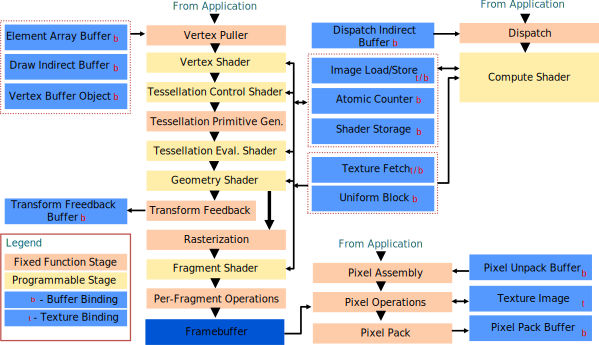
\includegraphics[width=10cm,keepaspectratio]{pics/opengl43.pdf}
	\end{figure}
\end{frame}

\begin{frame}
\frametitle{Compute Shader}
	\begin{figure}[h]
	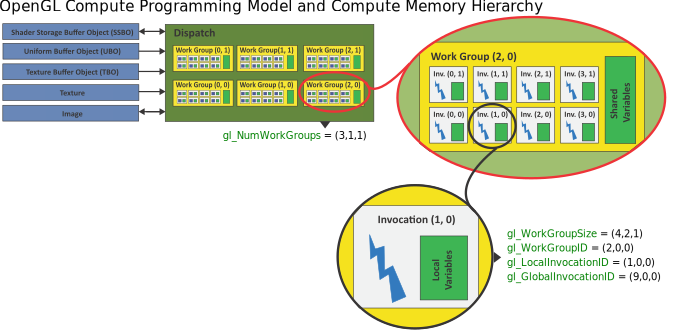
\includegraphics[width=11cm,keepaspectratio]{pics/compute.pdf}
	\end{figure}
\end{frame}

\begin{frame}[fragile]
\frametitle{Compute Shader - example}
	{\scriptsize
	\begin{minted}[frame=lines]{glsl}
#version 430

layout(binding=0)buffer Input{vec4 i[];};//input buffer
layout(binding=1)buffer Output{vec4 o[];};//output buffer
layout(local_size_x=32,local_size_y=1,local_size_z=1)in;//work-group size

uniform uint num;//number of elements in buffers

void main(){
  //gl_GlobalInvocationID = gl_WorkGroupID*gl_WorkGroupSize + gl_LocalInvocationID	
  uint gid = gl_GlobalInvocationID.x;
  if(gid >= num)return;
  vec3 v = i[gid].xyz;
  o[gid] = vec4(normalize(v),length(v));
}
	\end{minted}
	}
\end{frame}

\begin{frame}[fragile]
\frametitle{Compute Shader - example}
	{\scriptsize
	\begin{minted}[frame=lines]{c++}
uint32_t num=100;
GLuint CompBufferInput;
glCreateBuffers(1,&CompBufferInput);
glNamedBufferData(CompBufferInput,sizeof(float)*4*num,nullptr,GL_STATIC_DRAW);

GLuint CompBufferOutput;
glCreateBuffers(1,&CompBufferOutput);
glNamedBufferData(CompBufferOutput,sizeof(float)*4*num,nullptr,GL_DYNAMIC_COPY);

glBindBufferBase(GL_SHADER_STORAGE_BUFFER,0,CompBufferInput);
glBindBufferBase(GL_SHADER_STORAGE_BUFFER,1,CompBufferOutput);

glUseProgram(ComputeShader);
glUniform1ui(glGetUniformLocation(ComputeShader,"num"),num);

uint32_t workGroupSize = 32;

glDispatchCompute(divRoundUp(num,workGroupSize),1,1);
	\end{minted}
	}
\end{frame}

\begin{frame}[fragile]
\frametitle{Compute Shader - dispatch synchronization}
  \begin{itemize}
    \item Synchronization needs to be done between two shaders thats operates on same data.
    \item Synchronization is performed using glMemoryBarrier(); command.
  \end{itemize}

	{\scriptsize
	\begin{minted}[frame=lines]{c++}
//This compute shader creates buffer with vertices.
glDispatchCompute(
    this->TileCount[(this->NumLevels-2)*2+0],
    this->TileCount[(this->NumLevels-2)*2+1],
    1);

//Wait for modification to SSBO
glMemoryBarrier(GL_SHADER_STORAGE_BARRIER_BIT);

//Draw generated vertices
glDrawArrays(...)
	\end{minted}
	}
\end{frame}

\begin{frame}[fragile]
\frametitle{Compute Shader - thread synchronization}
  \begin{itemize}
    \item Threads in work-group are execute in warp/wavefronts.
    \item We can synchronize threads that are part of work-group.
    \item We cannot synchronize threads that are part of different work-groups.
    \item Threads that are part of warp do not have to be synchronized.
    \item Synchronization is performed by barrier() command.
    \item A barrier command has to lie on program path that can be access by all threads in work-group.
    \item A barrier command stops every thread until all other threads in work-group reach it.
  \end{itemize}
  Example:
	{\scriptsize
	\begin{minted}[frame=lines]{glsl}
layout(std430,binding=0)readonly buffer SFData{float data[];};
shared float array[size];
void main(){
  //cooperative reading from global memory into local/shared memory.
  array[gl_LocalInvocationID.x]=data[gl_GlobalInvocationID.x];
  //wait for all threads
  barrier();
  //...
}
	\end{minted}
	}
\end{frame}


\bluepage{Queries, Debugging}

\begin{frame}
\frametitle{Queries}
	\begin{itemize}
	\item Queries can be used to obtain some information about drawing.
	\item Number of rasterized samples.
	\item Number of generated primitives.
	\item Time of execution of commands.
	\item Conditional rendering - occlusion culling
	\end{itemize}
	{\scriptsize
	\mint[bgcolor=bg]{packages/c_cpp.py:CppLexer -x}|void glGenQueries(GLsizei n,GLuint * ids);|
	\mint[bgcolor=bg]{packages/c_cpp.py:CppLexer -x}|void glBeginQuery(GLenum target,GLuint id);|
	\mint[bgcolor=bg]{packages/c_cpp.py:CppLexer -x}|void glEndQuery(GLenum target,GLuint id);|
	\mint[bgcolor=bg]{packages/c_cpp.py:CppLexer -x}|void glGetQueryiv(GLenum target,GLuint id,GLint * params);|
	}
\end{frame}

\begin{frame}[fragile]
\frametitle{Queries - time example}
{\scriptsize
\begin{minted}[bgcolor=bg]{packages/c_cpp.py:CppLexer -x}
//init
GLuint QueryTime;//query
glGenQueries(1,&QueryTime);//nagenerujeme si ID query
GLuint QueryTimePassed=0;//cas v nanosekundach

//start query
glBeginQuery(GL_TIME_ELAPSED,QueryTime);

//commands
//glBindBuffer(...);
//glUseProgram(...);
//glDrawArrays(...);
//...

//end query
glEndQuery(GL_TIME_ELAPSED);//vypneme query

//get data from asychronous  query
glGetQueryObjectuiv(QueryTime,GL_QUERY_RESULT_NO_WAIT,&QueryTimePassed);
\end{minted}
}
\end{frame}

\begin{frame}[fragile]
\frametitle{Queries - conditional rendering example}
{\scriptsize
\begin{minted}[bgcolor=bg]{packages/c_cpp.py:CppLexer -x}
//init
GLuint QuerySample;//query
glGenQueries(1,&QueryTime);//nagenerujeme si ID query

//draw bounding boxes
//start query
glBeginQuery(GL_ANY_SAMPLES_PASSED,QuerySample);
//draw bounding boxes 
//glBindBuffer(...);
//glUseProgram(...);
//glDrawArrays(...);
//...
glEndQuery(GL_ANY_SAMPLES_PASSED);//vypneme query

//conditional rendering
//start conditional rendering
glBeginConditionalRender(QuerySample,GL_QUERY_NO_WAIT);
//draw meshes with full details
//glBindBuffer(...);
//glUseProgram(...);
//glDrawArrays(...);
//...
glEndConditionalRender();//end conditional rendering
\end{minted}
}
\end{frame}

\begin{frame}[fragile]
\frametitle{Synchronization objects, fences}
  \begin{itemize}
    \item Synchronization between OpenGL commands.
    \item Host synchronization, client synchronization.
  \end{itemize}
{\scriptsize
\begin{minted}[bgcolor=bg]{packages/c_cpp.py:CppLexer -x}
GLsync sync;//synchronization object
glDispatchCompute(...);
sync=glFenceSync(GL_SYNC_GPU_COMMANDS_COMPLETE,0);
glClientWaitSync(sync,0,GL_TIMEOUT_IGNORED);//CPU waits
//...
glDeleteSync(sync);
\end{minted}
}
{\scriptsize
\begin{minted}[bgcolor=bg]{packages/c_cpp.py:CppLexer -x}
GLsync sync;//synchronization object
glDispatchCompute(...);
sync=glFenceSync(GL_SYNC_GPU_COMMANDS_COMPLETE,0);
glWaitSync(sync,0,GL_TIMEOUT_IGNORED);//GPU waits
//...
glDeleteSync(sync);
\end{minted}
}
{\scriptsize
\begin{minted}[bgcolor=bg]{packages/c_cpp.py:CppLexer -x}
glFlush();
glFinish();
\end{minted}
}
\end{frame}


\begin{frame}
\frametitle{Debug}
	\begin{itemize}
	\item OpenGL exposes commands for debugging.
	\item User can define custom messages, callbacks, ...
	\item Old way: \textcolor{blue}{glGetError}
	\item OpenGL debugging is supported in debug OpenGL context
	\end{itemize}
	{\scriptsize
	\mint[bgcolor=bg]{packages/c_cpp.py:CppLexer -x}|void glDebugMessageCallback(DEBUGPROC callback,void * userParam);|
	\mint[bgcolor=bg]{packages/c_cpp.py:CppLexer -x}|void glDebugMessageControl(GLenum,GLenum,GLenum,GLsizei,const GLuint*,...);|
	\mint[bgcolor=bg]{packages/c_cpp.py:CppLexer -x}|void glDebugMessageInsert(GLenum,GLenum,GLuint,GLenum,GLsizei,const char*);|
	}
\end{frame}

\begin{frame}[fragile]
\frametitle{Debugging - example}
Debug context initialization.
{\scriptsize
\begin{minted}[bgcolor=bg]{packages/c_cpp.py:CppLexer -x}
//create window using SDL2
SDL_Init(SDL_INIT_VIDEO|SDL_INIT_TIMER);//init. video
SDL_GL_SetAttribute(SDL_GL_CONTEXT_MAJOR_VERSION,4);
SDL_GL_SetAttribute(SDL_GL_CONTEXT_MINOR_VERSION,3);
SDL_GL_SetAttribute(SDL_GL_CONTEXT_PROFILE_MASK,
  SDL_GL_CONTEXT_PROFILE_CORE);
//set debug context
SDL_GL_SetAttribute(SDL_GL_CONTEXT_FLAGS,SDL_GL_CONTEXT_DEBUG_FLAG);
SDL_CreateWindow("OpenGL with debug context",SDL_WINDOWPOS_CENTERED,
  SDL_WINDOWPOS_CENTERED,1024,768,
  SDL_WINDOW_OPENGL|SDL_WINDOW_SHOWN|SDL_WINDOW_FULLSCREEN);
\end{minted}
}
Setting up a debug callback.
{\scriptsize
\begin{minted}[bgcolor=bg]{packages/c_cpp.py:CppLexer -x}
//custom callback
void MyDebug(GLenum Source,GLenum Type,GLuint Id,GLenum severity,
  GLsizei Length,const GLchar*Message,void*UserParam){
    std::cerr<<"MyDebug: "<<Message<<std::endl;
}

glEnable(GL_DEBUG_OUTPUT);//enable debugging
glDebugMessageCallback(MyDebug,NULL);//set callback
\end{minted}
}
\end{frame}





\begin{frame}
\frametitle{Zdroje informací}
    \begin{itemize}
    \item \url{https://www.opengl.org/sdk/docs/man/}
    \item \url{www.khronos.org/files/opengl45-quick-reference-card.pdf}
		\item \url{http://www.opengl.org/documentation/glsl/}
    \item \url{http://www.geeks3d.com/20140321/opengl-approaching-zero-driver-overhead/}
    \end{itemize}
\end{frame}

\begin{frame}
\frametitle{Konec}
    \begin{center}
    Děkuji za pozornost\\
    \vspace{10 mm}
    Otázky?
    \end{center}
\end{frame}

\end{document}


